\documentclass[a5paper]{book}

\setlength\marginparwidth{30pt}

\usepackage[utf8]{inputenc}
\usepackage{t1enc}
\def\magyarOptions{defaults=hu-min}
\usepackage[magyar]{babel}
\addto\captionsmagyar{\renewcommand{\chaptername}{lecke}}

\usepackage[dvipsnames]{xcolor}
\usepackage{amsmath}
\usepackage{amsthm}
\usepackage{enumitem}
\usepackage{fancyvrb}
\usepackage[symbol]{footmisc}
\usepackage[all]{genealogytree}
\usepackage{imakeidx}
\usepackage{pdfpages}
\usepackage{storebox}
\usepackage{tcolorbox}

% Layout for debugging
%\usepackage{showframe}

\makeindex[intoc]

% Definitions
\renewcommand{\thefootnote}{\fnsymbol{footnote}}
\renewcommand{\thempfootnote}{\fnsymbol{mpfootnote}}
\newenvironment{program}{
  \VerbatimEnvironment
  \begin{Verbatim}[frame=leftline,numbers=left,formatcom=\color{OliveGreen}]}{\end{Verbatim}
}
\newenvironment{query}{
  \VerbatimEnvironment
  \begin{Verbatim}[frame=leftline,formatcom=\color{Violet}]}{\end{Verbatim}
}
\newcommand{\pr}[1]{{\tt #1}}
\newcommand{\name}[1]{{\sc #1}}
\theoremstyle{definition}
\newtheorem{problem}{Feladat}
\newenvironment{infobox}[2]{
  \begin{tcolorbox}[center,
                    float,
                    floatplacement=ht!,
                    fonttitle=\sffamily\bfseries,
                    title={\center Kitérő: \emph{#2}},
                    width=#1\linewidth]
  }{
  \end{tcolorbox}
}

\begin{document}

\frontmatter
\pagenumbering{roman}

% Cover page
\includepdf{images/cover.pdf}

% Inside cover
\thispagestyle{empty}
\newpage

% Flyleaf
\begin{titlepage}
\thispagestyle{empty}
\centering
\vspace*{2cm}
{\large OLDD MEG PROLOGBAN!}
\end{titlepage}

% Inside cover
\thispagestyle{empty}
\newpage

% Title page
\begin{titlepage}
\centering
\vspace*{2cm}
{\Large OLDD MEG PROLOGBAN!}\\
\vspace{8cm}
{\large Salvi Péter}\\
\vspace{1em}
2022
\end{titlepage}

% Kolofon
\thispagestyle{empty}
\begin{center}
  \small
  Salvi Péter: Oldd meg Prologban!\\
  Budapest, 2022 (\input{revision}verzió)\\
  \bigskip
  A könyv a Creative Commons \emph{Share Alike} licencnek megfelelően
  szabadon terjeszthető.
\end{center}
\vspace*{\fill}
{\footnotesize Ez a könyv \LaTeX-ben készült, Computer Modern betűtípussal.\\
  A borítón egy Lindenmayer-rendszer, az ún.~\emph{sárkány görbe} látható.
}

% Ajanlas
\clearpage
\thispagestyle{empty}
\begin{center}
  \vspace*{\fill}
  {\Large\emph{Zsófinak és Julinak}}
  \vspace*{\fill}
\end{center}
\clearpage

\thispagestyle{empty}
\newpage

\addtocounter{page}{2}

\tableofcontents

\chapter{Előszó}
Ez a könyv elsősorban azoknak szól, akik még egyáltalán nem tudnak
programozni, de szeretnék megismerni a számítógépes problémamegoldás
alapjait. A ,,programozás'' ma már egy rendkívül szerteágazó
gyűjtőfogalommá vált, melynek egy-egy területe magában egy-egy szakmát
képvisel. Itt nem lesz szó webfejlesztésről, látványos játékokról vagy
neurális hálókról: kizárólag a problémamegoldásra fogunk koncentrálni,
ami viszont -- az én véleményem szerint -- a programozás
legizgalmasabb válfaja.

Ehhez a Prologot fogjuk használni. Ez az 50 éves múltra visszatekintő
programozási nyelv sokáig állt a mesterséges intelligencia kutatás
középpontjában, és bár az iparban nem hódított teret, az informatika
oktatásában továbbra is jelentős szerepe van. Ez nem véletlen: a
Prolog különösen alkalmas tanításra, ugyanis egészen minimális
ismeretekkel is már érdekes feladatok megoldását teszi lehetővé. Ezt
bizonyítják az egyes leckéket lezáró \emph{projektek} is, amelyekben
különböző, kicsit nagyobb lélegzetvételű problémákat vizsgálunk majd
meg.

\section*{Hogyan használjuk a könyvet?}
A leckékben szereplő példákat érdemes a számítógépen kipróbálni, és
kísérletezgetni velük, átírni bennük ezt--azt, és megvizsgálni, hogy mi
történik. Az efféle játék során mélyül el igazán a tudás; és ezt
segítik a feladatok is, melyeknek megoldása a könyv végén található.

Mindehhez természetesen szükség van egy Prolog fordítóra. Ezekből sok
létezik, és mindegyik meglehetősen különböző. A legtöbb azonban
kompatibilis az 1995-ös ISO szabvánnyal, és ez a könyv csak ezt
feltételezi, illetve még annyit, hogy tudja kezelni a magyar ábécé
betűit. Az ingyenesen letölthető, nyílt forráskódú rendszerek közül
ilyen az \name{SWI-Prolog}. Más implementációk, mint pl. az~\name{XSB}
vagy a \name{GNU Prolog}, jelenleg nem fogadják el az ékezetes
karaktereket, ezért ezek használata esetén a programokat ékezetek
nélkül kell begépelni.

A problémamegoldás Prologban mindig két részből áll:
\begin{enumerate}
\item Egy -- általában {\tt .pl} vagy {\tt .P} kiterjesztésű --
  fájlban megadunk egy szabályrendszert (a program
  \emph{forráskódját}). Ennek megírásához tetszőleges
  szövegszerkesztőt használhatunk.\index{forráskód}
\item Ezzel kapcsolatban a programnak felteszünk kérdéseket.
\end{enumerate}
A legtöbb Prolog rendszer indításkor mindössze egy kérdőjel kiírásával
fogad minket; ezzel jelzi, hogy várja a kérdést:
\begin{query}
?-
\end{query}  
Az első feladatunk, hogy betöltsük az általunk írt programot. Ezt
általában a \pr{consult} paranccsal tehetjük meg, például:\index{\pr{consult}}
\begin{query}
?- consult('/home/salvi/szabályok.pl').
\end{query}
\dots ahol az aposztrófok között levő {\tt /home/salvi/szabályok.pl} a
forráskód teljes elérési útja. Ne felejtsük le a parancs végéről a
pontot, majd nyomjuk meg az újsor billentyűt.

Ezután már jöhetnek a kérdések. A leckékben már csak ezek lesznek
feltüntetve, de nem szabad megfeledkezni a szabályok betöltéséről sem.
Amennyiben egy kérdésre több válasz is van, a következő választ
általában a pontosvessző ({\tt ;}) lenyomásával kaphatjuk meg, a
következő kérdés feltevéséhez pedig ilyenkor egy újsor billentyűt kell
nyomni.

Bizonyos rendszerekben mindez kényelmesebben is megtehető, így pl.~az
\name{SWI-Prolog} internetes \name{SWISH} verziójában,\footnote{\tt
https://swish.swi-prolog.org/} ahol a szabályok mindig automatikusan
újraolvasódnak.

\section*{Források}
Ezt a könyvet eredetileg azzal a céllal kezdtem el, hogy az egyik
kedvenc programozásról szóló könyvemet~[1] elérhetőbbé és köny-nyebben
emészthetővé tegyem a magyar laikus közönség számára. Ez aztán végül
egy Prolog tankönyvvé vált, de a leckék -- helyenként jelentősen
átdolgozva -- az eredetit követik. Egészen pontosan az 1.~lecke az
1.1--3 és 1.8, a 2.~lecke a 2.1--6, a 3.~lecke a 3.1--2, a 4.~lecke a
3.3--4, az 5.~lecke az 5.1--4 és 9.1, a 6.~lecke pedig a 6.1--6 és 8.5
fejezeteknek felel meg.

Egy másik fontos forrás egy klasszikus Prolog tankönyv~[2]; ebből
származik az 5.~lecke összefésüléses példája (11.~fejezet), a
6.~leckében a különbség-listák tárgyalása (15.1 fejezet), és a
lecke végén található projekt (20.2 és 21.3 fejezetek).

A 7.~lecke alapját képező forráskód az \name{SWI-Prolog}
szoftvercsomag része.

\begin{itemize}[leftmargin=2cm,itemindent=-1cm,labelsep=1cm-2em]
\item[{[1]}] I.~Bratko: \emph{Prolog Programming for Artificial
Intelligence}, 4th Ed., Pearson, 2011.
\item[{[2]}] L.~Sterling, E.~Shapiro, \emph{The Art of Prolog}, 2nd
  Ed., MIT Press, 1994.
\end{itemize}

\section*{Köszönetnyilvánítás}
Köszönettel tartozom mindenekelőtt Varga Csillának, aki lelkesen
végigcsinálta a könyvnek egy korai változatát, és kérdéseivel
rávilágított arra, hogy mit kell még pontosítanom vagy jobban
elmagyaráznom; és természetesen a feleségemnek, Iida Norikónak, akinek
a támogatása nélkül ez a könyv nem készülhetett volna el.

\begin{flushright}
  Salvi Péter\\
  Budapest, 2022.
\end{flushright}


\mainmatter
\pagenumbering{arabic}

% -*- fill-column: 52 -*-
% (local-set-key (kbd "C-c C-f") 'display-fill-column-indicator-mode)

\chapter{Tények és szabályok}
Az első leckében egy családfa vizsgálatán keresztül
megismerkedünk a programok alkotóelemeivel és a
\emph{rekurzió}\/val.

\subsection*{Tények}
Egy Prolog program \emph{tényekből} és
\emph{szabályokból} áll, amelyekből a számítógép
következtetéseket tud levonni. Ha megadunk egy tény-
és szabályrendszert, utána kérdéseket tehetünk fel,
amelyeket a gép legjobb tudása szerint megválaszol.

Példaként vegyük Mohamed próféta családját
(\ref{fig:csaladfa}.~ábra)!
%
\begin{figure}
  \centering
  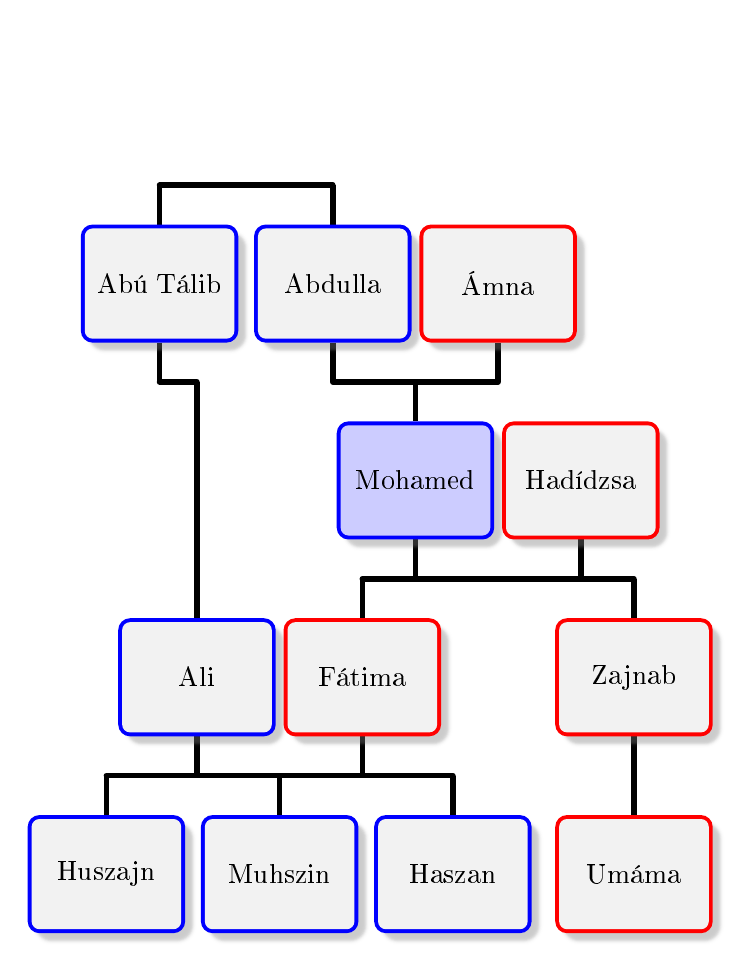
\begin{tikzpicture}
    \gtrset{edges={foreground={line width=2pt,black},no background}}
    \genealogytree[template=signpost,
                   options for node=m{box={colback=blue!20}},
                   options for family={af}{extra edges=ta{foreground={line width=2pt,black}}}]{
      child {
        g[male,phantom]{Valaki}
        c[male,id=t]{\large Abú Tálib}
        child[id=af] {
          g[male]{\large Abdulla}
          p[female]{\large Ámna}
          child {
            g[male,id=m]{\large Mohamed}
            p[female]{\large Hadídzsa}
            child {
              p[male,id=a]{\large Ali}
              g[female]{\large Fátima}
              c[male]{\large Huszajn}
              c[male]{\large Muhszin}
              c[male]{\large Haszan}
            }
            child {
              g[female]{\large Zajnab}
              c[female]{\large Umáma}
            }
          }
        }
      }
    }
  \end{tikzpicture}
  \caption{Mohamed próféta családja (részlet).}
  \label{fig:csaladfa}
\end{figure}
%
A szülő--gyerek kapcsolatokat az alábbi program
foglalja össze:

\begin{program}
szülő(abú_tálib, ali).
szülő(abdulla, mohamed).
szülő(ámna, mohamed).
szülő(mohamed, fátima).
szülő(hadídzsa, fátima).
szülő(mohamed, zajnab).
szülő(hadídzsa, zajnab).
szülő(ali, huszajn).
szülő(fátima, huszajn).
szülő(ali, muhszin).
szülő(fátima, muhszin).
szülő(ali, haszan).
szülő(fátima, haszan).
szülő(zajnab, umáma).
\end{program}

Ebben a programban minden sor egy \emph{tény}. Egy
tény dolgok (itt emberek) közti kapcsolatot ír le. A
formája a következő: a kapcsolat nevével kezdődik
(most ez a \pr{szülő}), utána zárójelek között
vesszővel elválasztva felsoroljuk a kapcsolatban
levő dolgokat, és a végén egy ponttal (\pr{.})
zárjuk.\index{teny@tény}

Talán furcsa lehet, hogy minden kisbetűvel szerepel --
majd később lesz szó arról, hogy mik az elnevezés
pontos szabályai, egyelőre azt jegyezzük meg, hogy
minden \emph{konkrét} dolog kisbetűvel írandó, és
nem lehet benne szóköz.

\begin{infobox}{}{Mohamed családfája}
A programban a családfának csak egy nagyon kis
szeletét használtuk, és még ezen a részen belül
sem tartalmaz minden kapcsolatot, mert pl.~Ali
Fátima halála után feleségül vette Umámát is.

\begin{center}
  \includegraphics[width=.75\textwidth]{images/prophet-family.jpg}
\end{center}
\end{infobox}

\subsection*{Egyszerű kérdések}

Már egy ilyen egyszerű program esetén is lehet
értelmes kérdéseket feltenni. Például
megkérdezhetjük, hogy
\begin{query}
?- szülő(mohamed, fátima).
\end{query}
\dots amire a rendszer a \pr{true} (igaz) vagy
\pr{yes} (igen) üzenettel
válaszol;\index{\pr{true}}\index{\pr{yes}} vagy hogy
\begin{query}
?- szülő(ali, zajnab).
\end{query}
\dots amire a \pr{false} (hamis) vagy \pr{no} (nem)
eredményt adja.\index{\pr{false}}\index{\pr{no}} (A
továbbiakban ez a könyv a \pr{true} és \pr{false}
válaszokat fogja használni.)

Egy kicsit érdekesebb a következő kérdés:
\begin{query}
?- szülő(mohamed, Kicsoda).
\end{query}
Erre azt a feleletet kapjuk, hogy \pr{Kicsoda =
  fátima}. Ha további válaszokat kérünk, akkor még
azt is megmondja, hogy \pr{Kicsoda = zajnab}.

Mi történt itt? Azáltal, hogy a második helyre egy
nagybetűs szót (\pr{Kicsoda}) írtunk, azt mondtuk,
hogy ez egy határozatlan, ismeretlen érték, egy
\emph{változó}.\index{valtozo@változó} A kérdést tehát
magyarul úgy lehetne megfogalmazni: ,,Mohamed kinek
a szülője?''

Erre megkeresi az első választ, amit talál
(\pr{fátima}), és ha továbbit kérünk tőle, akkor
megtalálja \pr{zajnab}ot is, és látja, hogy nincs
több, és így leáll.

Ha kisbetűvel írtuk volna:
\begin{query}
?- szülő(mohamed, kicsoda).
\end{query}
\dots akkor a \pr{false} eredményt kaptuk volna,
hiszen \pr{kicsoda} itt egy konkrét dolgot jelöl, a
kérdés tehát azt jelenti: ,,Igaz-e, hogy Mohamed
szülője Kicsodának?''

A kérdés a másik irányban is feltehető:
\begin{query}
?- szülő(Ki, ali).
\end{query}
\dots tehát ,,Ki Ali szülője?'', amire a \pr{Ki =
  abú\_tálib} feleletet kapjuk.

Még tovább is mehetünk, és rákérdezhetünk az összes
szülő-gyerek kapcsolatra:
\begin{query}
?- szülő(Ki, Kinek).
\end{query}
\dots azaz ,,Ki kinek a szülője?''. Az első válasz
az lesz, hogy
\begin{query}
Ki = abú_tálib,
Kinek = ali
\end{query}
További válaszok kérésével sorban megkapjuk az
adatbázisunk minden egyes elemét.

\subsection*{Összetett kérdések}

Tegyük fel, hogy arra vagyunk kíváncsiak, hogy kik
Mohamed unokái. Hogyan tudjuk ezt megkérdezni? Az
unoka definíció szerint a gyerek gyereke, tehát
tudjuk, hogy van valaki, aki szülője az unokának, és
akinek a szülője Mohamed. A logikai \emph{és}\/sel
összekötött, együtt teljesítendő feltételeket
vesszővel választjuk el:
\begin{query}
?- szülő(mohamed, Valaki), szülő(Valaki, Unoka).
\end{query}
Négy megoldást is kapunk:
\begin{query}
Unoka = huszajn,
Valaki = fátima ;
Unoka = muhszin,
Valaki = fátima ;
Unoka = haszan,
Valaki = fátima ;
Unoka = umáma,
Valaki = zajnab
\end{query}
(Ezek páronként értendők, tehát Fátimától van
Huszajn, Muhszin és Haszan, és Zajnabtól Umáma.)

Ez azért működik, mert egy változónak minden
előfordulása azonos értéket kell, hogy kapjon,
tehát a két \pr{szülő}s kifejezésben a \pr{Valaki}
ugyanarra vonatkozik.
A kérdés két tagjának sorrendje felcserélhető, tehát
ugyanezt az eredményt adja ez is:
\begin{query}
?- szülő(Valaki, Unoka), szülő(mohamed, Valaki).
\end{query}
(Majd látni fogjuk viszont, hogy a számításigényük
nem azonos, érdemesebb az erősebb megszorítással
kezdeni.)

Hasonlóan rákérdezhetünk, hogy kik Huszajn
nagyszülei:
\begin{query}
?- szülő(Valaki, huszajn), szülő(Nagyszülő, Valaki).
\end{query}
\dots amire megkapjuk Abú Tálibot, Mohamedet és
Hadídzsát.

Ha arra vagyunk kíváncsiak, hogy Haszan testvére-e
Huszajnnak, így fogalmazhatjuk meg:
\begin{query}
?- szülő(Valaki, haszan), szülő(Valaki, huszajn).
\end{query}
Azt kapjuk, hogy \pr{Valaki = ali}, tehát a válasz
igen. Ha \pr{huszajn} helyett \pr{abdullá}t írunk,
akkor \pr{false} választ kapunk.

\begin{problem}
Válaszold meg az alábbi kérdéseket!
\begin{query}
?- szülő(huszajn, X).
?- szülő(X, huszajn).
?- szülő(ámna, X), szülő(X, fátima).
?- szülő(ámna, X), szülő(X, Y), szülő(Y, haszan).
\end{query}
\end{problem}
\begin{problem}
Fogalmazd meg Prologban!
\begin{enumerate}
\item Ki Ali szülője?
\item Umámának van gyereke?
\item Ki Zajnab nagyszülője?
\end{enumerate}
\end{problem}
\begin{problem}
Készítsd el a saját családfádat (nagyszülőkig
és unokatestvérekig)!
\end{problem}

\begin{infobox*}{}{\pr{false} = nincs több megoldás}
A Prolog gyakran olyankor is felajánlja a
további megoldások keresését, amikor nincs több --
egyszerűen azért, mert még \emph{ő} sem tudja.
Ha ezután mégiscsak kiderül, hogy nincs más
megoldás, akkor ezt \pr{false}-szal
jelzi. Bizonyos esetekben ez megkerülhetetlen,
máskor az adott rendszertől függ, hogy észreveszi-e,
hogy felesleges a további keresés.
\end{infobox*}

\subsection*{Szabályok}

Eddig csak tényekkel foglalkoztunk, de valójában a
Prolog programok nagy része \emph{szabályokból}
áll. Először is egészítsük ki a programunkat a
szereplőink nemével!\index{szabály}

\begin{program}
férfi(abú_tálib).
férfi(abdulla).
férfi(mohamed).
férfi(ali).
férfi(huszajn).
férfi(muhszin).
férfi(haszan).

nő(ámna).
nő(hadídzsa).
nő(fátima).
nő(zajnab).
nő(umáma).
\end{program}

Ha most a \pr{szülő} mellett szeretnénk \pr{anya} és
\pr{apa} kapcsolatokat is létrehozni, ezt
megtehetjük egyenként:
\begin{program}
anya(ámna, mohamed).
anya(hadídzsa, fátima).
...
apa(abú_tálib, ali).
apa(abdulla, mohamed).
...
\end{program}
Ez azonban elég sok munka, és érezzük, hogy
felesleges, hiszen kikövetkeztethető.  Szabályok
segítségével ezt sokkal egyszerűbben megoldhatjuk:
\begin{program}
anya(X, Y) :- szülő(X, Y), nő(X).
apa(X, Y) :- szülő(X, Y), férfi(X).
\end{program}
A \pr{:-} jelet itt úgy olvashatjuk ki, hogy
,,akkor, ha'', tehát ,,X anyja Y-nak akkor, ha X
szülője Y-nak és X nő''. A baloldalon levő részt a
szabály \emph{fej}\/ének, a jobboldalát a szabály
\emph{törzs}\/ének nevezzük.
\index{\pr{:-}}\index{fej}\index{torzs@törzs}

Mi történik, amikor feltesszük az alábbi kérdést?
\begin{query}
?- anya(ámna, mohamed).
\end{query}
A rendszer megtalálja az \pr{anya} szabályt, és
\emph{egyesíti} az \pr{X}-et \pr{ámná}\-val, az
\pr{Y}-t pedig \pr{mohamed}del.\index{egyesítés} (Az
egyesítésről még később szó lesz, itt egyszerűen
helyettesítést jelent.) Ezután megnézi, hogy a
szabály jobboldalán levő feltétel teljesül-e; ez
most a
\begin{query}
szülő(ámna, mohamed), nő(ámna).
\end{query}
\dots és ezek a tények szerepelnek a programban,
tehát \pr{true} válasszal tér vissza.

Definiáljuk a ,,nagyszülő'' kapcsolatot!
\begin{program}
nagyszülő(X, Z) :- szülő(X, Y), szülő(Y, Z).
\end{program}
Ez pontosan követi azt, ahogy korábban megkerestük
valakinek a nagyszülőjét.

\subsection*{Problémás esetek}

Hogyan tudnánk megadni a ,,fivér'' kapcsolatot?
\begin{program}
fivér(X, Y) :- férfi(X), szülő(Z, X), szülő(Z, Y).
\end{program}
Tehát X fivére Y-nak, ha férfi és van közös
szülője Y-nal.

Itt érdemes megjegyezni, hogy bár Abú Tálib és
Abdulla testvérek voltak, a
\begin{query}
?- fivér(abú_tálib, abdulla).
\end{query}
kérdésre \pr{false} a válasz, mivel a programnak
nincs arról tudomása, hogy lenne közös szülőjük. (A
Prolog mindent hamisnak vesz, amit az általa ismert
adatokból nem tud kikövetkeztetni, és ez időnként
furcsa következményekkel járhat -- erről majd
később.)

Egy másik problémába ütközünk, ha Mohamed fivéreire
vagyunk kíváncsiak:
\begin{query}
?- fivér(mohamed, X).
\end{query}
Az eredmény, meglepő módon, \pr{X = mohamed}! Ebből
látszik, hogy a definíciónk nem volt elég pontos;
hozzá kell venni azt is, hogy senki nem fivére
önmagának:
\begin{program}
fivér(X, Y) :-
    férfi(X),
    szülő(Z, X), szülő(Z, Y),
    X \= Y.
\end{program}
Itt a \pr{\textbackslash=} jelentése ,,nem azonos''.
\index{\pr{\textbackslash=}} Ez a példa azt is
illusztrálja, hogy a szabályok több sorban is
írhatóak; ilyenkor a második és további sorokat
beljebb szokás húzni.

\begin{infobox*}{}{Többszörös megoldások}
A ,,\pr{?- fivér(huszajn, muhszin).}'' kérdésre
érdekes módon két \pr{true} választ kapunk.
Ennek az az oka, hogy a fivéri kapcsolatot
kétféleképpen is be lehet bizonyítani, Alin és
Fátimán keresztül.
\end{infobox*}

\subsection*{Egyedüli változók}

Készítsük el a
\begin{program}
vangyereke(X) :- szülő(X, Y).
\end{program}
szabályt.  Ennek az az érdekessége, hogy attól
függően, hogy hogyan olvassuk ki, az állítás
\emph{minden} Y-ra vonatkozik, vagy csak azt
mondja, hogy \emph{létezik} egy fajta Y:

\begin{enumerate}
\item (Minden X és Y esetén,) ha X szülője Y-nak,
  akkor X-nek van gyereke.
\item X-nek akkor van gyereke, ha létezik olyan Y,
  hogy X szülője Y-nak.
\end{enumerate}
A két olvasat egyenértékű; ez a kettősség annak a
következménye, hogy az \pr{Y} változó csak a szabály
törzsében fordul elő.

A fenti példa más miatt is érdekes. Mivel az \pr{Y}
változó a szabályban mindössze egyszer fordul elő,
nem lehet hatással az eredmény kiszámítására, tehát
érdektelen. Ezt úgy szokás jelezni, hogy a helyére
egy alsóvonást (\pr{\_}) írunk, vagy egy ezzel
kezdődő nevet (pl.~\pr{\_Y}).\index{\pr{\_}} Ha
kérdésben szerepel ilyen változó, akkor a válaszban
ennek az értéke nem fog megjelenni. Így pl.~az
alábbi kérdés megadja Mohamed unokáit anélkül, hogy
megmutatná a szülőket:
\begin{query}
?- szülő(mohamed, _Valaki), szülő(_Valaki, Unoka).
\end{query}

Ha több alsóvonás szerepel, ezek értéke lehet
különböző, tehát a
\begin{query}
?- szülő(_, _).
\end{query}
kérdésre \pr{true} lesz a válasz, pedig senki sem
szülője önmagának.

Ha egy egyszer szereplő változónak ,,normális''
nevet adunk, akkor erre a fordító általában
figyelmeztet minket, mert ez gyakran egy elírás
következménye. Pl.~az alábbi programban a
\pr{Valaki} változóból egyszer kimaradt egy \pr{a}
betű:
\begin{program}
nagyszülő(X, Y) :-
    szülő(X, Valaki), szülő(Valki, Y).
\end{program}

\begin{problem}
Fordítsd le Prologra!
\begin{enumerate}  
\item Akinek van gyereke, az boldog. (\pr{boldog}
  szabály)
\item Minden X-re, ha X-nek van egy gyereke akinek
  van egy fivére, akkor X-nek két gyereke
  van. (\pr{kétgyerekes} szabály)
\end{enumerate}
\end{problem}
\begin{problem}
  Készítsd el az \pr{unoka} szabályt!
  Teszteld a saját családfádon!
\end{problem}
\begin{problem}
  Írj egy \pr{nagynéni} szabályt a \pr{szülő}
  és \pr{nővér} segítségével, és keresd meg vele
  Zajnab unokaöccseit!
\end{problem}

\section{Rekurzió}
Adjunk még egy utolsó szabályt a programunkhoz: az
\emph{ős} fogalmát. Valakinek az őseit úgy kapjuk
meg, hogy felfelé megyünk a családfában: ős a szülő,
a nagyszülő, a dédszülő stb. Ezt elkezdhetjük írni
szabályokkal:
\begin{program}
ős(X, Z) :- szülő(X, Z).
ős(X, Z) :- szülő(X, Y), szülő(Y, Z).
ős(X, Z) :-
    szülő(X, Y1), szülő(Y1, Y2), szülő(Y2, Z).
ős(X, Z) :-
    szülő(X, Y1), szülő(Y1, Y2),
    szülő(Y2, Y3), szülő(Y3, Z).
...
\end{program}
Ez nagyon jól működik, de véges -- bármennyi ilyen
programsort írunk, mindig feljebb tudunk menni
eggyel a családfában, és azt már nem kezeli.

Egy kis trükkel meg tudjuk ezt oldani: azt mondjuk,
hogy ha X gyereke őse Z-nek, akkor X is őse Z-nek:
\begin{program}
ős(X, Z) :- szülő(X, Y), ős(Y, Z).
\end{program}
Az \pr{ős} így önmagára hivatkozik, más szóval
\emph{rekurzív}.\index{rekurzió}

Ez így magában még azonban nem elég, mert így ahhoz,
hogy valaki ős legyen, mindig valaki másnak is ősnek
kéne lennie, amit a végtelenségig kéne folytatnunk.
Valahol ennek meg kell állnia; ehhez elég
hozzávenni a legegyszerűbb esetet, vagyis azt,
amikor maga a szülő az ős:
\begin{program}
ős(X, Z) :- szülő(X, Z).
ős(X, Z) :- szülő(X, Y), ős(Y, Z).
\end{program}
Ez a kettő együtt már működik. X őse Z-nek, ha vagy
(i) X szülője Z-nek, vagy (ii) X szülője Y-nak és Y
őse Z-nek.

Próbáljuk is ki:
\begin{query}
?- ős(X, huszajn).
X = ali ;
X = fátima ;
X = abú_tálib ;
X = abdulla ;
X = ámna ;
X = mohamed ;
X = hadídzsa
\end{query}

\begin{problem}
Tegyük fel, hogy az \pr{ős} definícióját
megváltoztatjuk!
\begin{program}
ős(X, Z) :- szülő(X, Z).
ős(X, Z) :- szülő(Y, Z), ős(X, Y).
\end{program}
Jó ez így? Miért?
\end{problem}

\section*{A teljes program}

Ay alábbi programban szerepel minden tény és
szabály, amiről szó volt. A \pr{\%} jel megjegyzések
hozzáadására használható, a rendszer szempontjából a
\pr{\%}-tól jobbra levő szöveg érdektelen, mintha
ott sem lenne.\index{\pr{\%}}

\begin{program}
% szülő(X, Y) => X az Y szülője
szülő(abú_tálib, ali).
szülő(abdulla, mohamed).
szülő(ámna, mohamed).
szülő(mohamed, fátima).
szülő(hadídzsa, fátima).
szülő(mohamed, zajnab).
szülő(hadídzsa, zajnab).
szülő(ali, huszajn).
szülő(fátima, huszajn).
szülő(ali, muhszin).
szülő(fátima, muhszin).
szülő(ali, haszan).
szülő(fátima, haszan).
szülő(zajnab, umáma).

férfi(abú_tálib).
férfi(abdulla).
férfi(mohamed).
férfi(ali).
férfi(huszajn).
férfi(muhszin).
férfi(haszan).

nő(ámna).
nő(hadídzsa).
nő(fátima).
nő(zajnab).
nő(umáma).

anya(X, Y) :- szülő(X, Y), nő(X).   % X az Y anyja
apa(X, Y) :- szülő(X, Y), férfi(X). % X az Y apja

nagyszülő(X, Z) :- szülő(X, Y), szülő(Y, Z).

fivér(X, Y) :-
    férfi(X),
    szülő(Z, X), szülő(Z, Y),
    X \= Y.

vangyereke(X) :- szülő(X, _).

ős(X, Z) :- szülő(X, Z).
ős(X, Z) :- szülő(X, Y), ős(Y, Z).
\end{program}

\clearpage

\section{Projekt: a négyszín-tétel}
Mindössze négy szín elég ahhoz, hogy tetszőleges
térképen az országokhoz színeket rendeljünk úgy,
hogy minden országhatár két különböző színt
válasszon el. (Ez feltételezi, hogy az országok
mindig összefüggőek, tehát nincsen másik ország, ami
kettéválasztaná őket -- ez egy valódi térképnél
gyakran nem teljesül.)

Próbáljuk meg kiszínezni Európa egy szeletét!

\begin{center}
  \includegraphics[width=0.7\textwidth]{images/europe.pdf}
\end{center}

Jelölje \pr{t} azt, hogy két ország
\emph{találkozik}. A találkozáskor a színeknek
különbözőeknek kell lennie, tehát felvehetjük a
következő tényeket (egyelőre 2 színnel):
\begin{program}
t(piros, zöld). t(zöld, piros).
\end{program}
Ahhoz, hogy a térképünk megfeleljen a
követelményeknek, minden határnál teljesülnie kell
egy ilyen találkozásnak:
\begin{program}
térkép(DE, CH, IT, PL, CZ, AT, SI, HR, SK, HU) :-
    t(DE, PL), t(DE, CZ), t(DE, AT), t(DE, CH),
    t(CH, AT), t(CH, IT),
    t(IT, AT), t(IT, SI),
    t(PL, CZ), t(PL, SK),
    t(CZ, AT), t(CZ, SK),
    t(AT, SK), t(AT, HU), t(AT, SI),
    t(SI, HU), t(SI, HR),
    t(HR, HU),
    t(SK, HU).
\end{program}

\begin{infobox}{}{a négyszín-tétel}
Ez volt az első olyan matematikai tétel, amelynek
bizonyítását számítógéppel adták meg, és ezért sok
matematikus kezdetben nem is fogadta el
bizonyítottnak, és csak ,,négyszín-sejtésként''
hivatkoztak rá. Minden joguk megvolt rá: a több,
mint egy hónapon át futó 1976-os eredeti program
állítólag tele volt hibákkal. 20 évvel később
azonban egy sokkal hatékonyabb megoldást is
találtak, és 2004-ben egy tételbizonyító rendszer is
belátta, hogy az állítás mindig igaz.
\end{infobox}

Mivel a színekre vonatkozó szabályt mindkét
sorrendben felvettük, az országok sorrendje nem
számít, és így elég mindig csak az egyik verziót
felírni. Ha most megkérdezzük, hogy
\begin{query}
?- térkép(DE, CH, IT, PL, CZ, AT, SI, HR, SK, HU).
\end{query}
\dots akkor (nem túl meglepő módon) tagadó választ
kapunk. Vegyünk hozzá még egy színt!
\begin{program}
t(piros, kék). t(zöld, kék).
t(kék, piros). t(kék, zöld).
\end{program}
\dots még mindig nem elég. (Ez is elég világos -- ha
Ausztria pl.~piros, akkor a szomszédos országokat
körbejárva felváltva kéne zöldet és kéket kapnunk,
de páratlan számú ország van körülötte.)
Vegyük akkor hozzá a sárgát is!
\begin{program}
t(piros, sárga). t(zöld, sárga). t(kék, sárga).
t(sárga, piros). t(sárga, zöld). t(sárga, kék).
\end{program}
Ha most tesszük fel a kérdést, akkor már talál
megoldást:
\begin{query}
AT = PL = zöld,
CH = CZ = SI = kék,
DE = HR = IT = SK = piros,
HU = sárga
\end{query}
Az egyetlen szépséghibája, hogy Szlovénia kék lett,
és így egybefolyhat a tenger kékjével. Több
lehetőségünk is van:
\begin{itemize}
\item Lecseréljük a kéket egy másik színre
\item Addig kérünk további megoldásokat, amíg már
  egy tengerparti ország sem lesz kék színű
\item Felcseréljük a kék és sárga színeket
\end{itemize}

Tegyük fel, hogy szeretjük a kék színt, és nem
akarjuk lecserélni (egyébként is akkor már 5
szín kéne!), a másik két megoldás pedig nem elég
automatikus. Mit tehetünk?

Felvehetjük plusz ,,országként'' a tengert, és
megkövetelhetjük, hogy mindig kék legyen:
\begin{program}
térkép(DE, CH, IT, PL, CZ, AT, SI, HR, SK, HU) :-
    Tenger = kék,
    t(DE, PL), t(DE, CZ), t(DE, AT), t(DE, CH),
    t(CH, AT), t(CH, IT),
    t(IT, AT), t(IT, SI),
    t(PL, CZ), t(PL, SK),
    t(CZ, AT), t(CZ, SK),
    t(AT, SK), t(AT, HU), t(AT, SI),
    t(SI, HU), t(SI, HR),
    t(HR, HU),
    t(SK, HU),
    t(DE, Tenger), t(IT, Tenger), t(PL, Tenger),
    t(SI, Tenger), t(HR, Tenger).
\end{program}
Így már tökéletes megoldást kapunk.\index{\pr{=}}
(Az egyenlőségjellel (\pr{=}) két kifejezést tudunk
\emph{egyesíteni}, erről majd többet a következő
leckében.)

Megtehettük volna azt is, hogy a \pr{Tenger}ek
helyett egyszerűen \pr{kék}et írunk, és akkor
nincsen szükség a \pr{Tenger = kék} sorra sem, de
egy kicsit kevésbé olvasható lenne a
forráskód. Ilyen rövid programoknál még ez nem olyan
lényeges, de általában a programozásban fontos arra
törekedni, hogy ne csak a számítógép, hanem egy
másik ember (és pár hét múlva mi magunk) is
megértse, amit írtunk.

% -*- fill-column: 52 -*-
% (local-set-key (kbd "C-c C-f") 'display-fill-column-indicator-mode)

\chapter{Típusok és egyesítés}
Az első leckében megismertük a tényeket és
szabályokat, és kaptunk egy első képet arról, hogy
hogyan is néz ki egy Prolog program. A következőkben
azzal fogunk foglalkozni, hogy megvizsgáljuk az
alapvető alkotóelemeket, valamint a programok fő
mozgató rugóját, az \emph{egyesítést}.

A Prolog \emph{kifejezés}\/eknek négy típusa van:
atom, szám, változó vagy struktúra. Az egyes típusok
,,helyesírására'' más és más szabályok vonatkoznak
-- nézzük meg ezeket közelebbről!
\index{kifejezés}\index{tipus@típus}
\subsection*{Atomok}
Láttuk, hogy vannak ,,konkrét dolgok'', amelyeket
kisbetűvel í\-runk. Ezeket \emph{atom}\/oknak szokás
nevezni. Az atomok neve háromféleképpen képezhető:
\begin{enumerate}
\item Betűk, számok és az alsóvonás (\pr{\_})
  karakter kombinációja, de az első mindig egy
  kisbetű. Pl.: \pr{nil}, \pr{foo1}, \pr{bar\_42},
  \pr{baz\_\_}, \pr{ez\_1\_hosszú\_név}.
\item Különleges karakterek sorozata (ezekből lehet
  válogatni: \pr{\#\$\&*+-./:<=>?{@}\^{}\~{}}),
  pl.~\pr{.:.} vagy \pr{==>} vagy \pr{+}.
\item Aposztrófok közti karaktersorozat,
  pl. \pr{'Peti'} vagy \pr{'Abú Tálib'}.
\end{enumerate}
Az első fajtára már sok példát láttunk; a másodikról
majd később lesz szó; a harmadikat pedig jellemzően
akkor használjuk, ha nagybetűvel kezdődő vagy
szóközt tartalmazó nevet szeretnénk adni (ritka).

\begin{infobox}{}{foo--bar--baz}
A programozók előszeretettel használják a \pr{foo},
\pr{bar} és \pr{baz} neveket, amikor valamilyen
példát mutatnak, ahol maga a név nem
fontos. Hasonlóan, ha egy példában egy egész számot
kell választani, ez leggyakrabban a \pr{42} (a
\emph{Galaxis útikalauz stopposoknak} nyomán). Ilyen
és hasonló programozó-szubkultúrával kapcsolatos
érdekességekről rengeteget lehet olvasni a \emph{Zsargon
  fájl}\/ban,\footnote[2]{http://www.catb.org/jargon/html/}
nagyon szórakoztató olvasmány. (Sajnos csak angolul
hozzáférhető, de sokszor nem is igazán lehetne
lefordítani.)
\index{foo--bar--baz}
\index{zsargon fájl}
\end{infobox}

\subsection*{Számok}
A Prolog egész és valós számokat tud kezelni, a
megszokott jelölésekkel (de angol szokás szerint
a tizedesvessző helyett ponttal). A valós számoknál lehet
használni az ún.~\emph{exponenciális formát} is,
ahol egy \pr{e} betű után a 10 kitevője szerepel,
tehát pl.~ugyanazt a számot jelöli a \pr{1.23e5} és
\pr{123000.0}, vagy a \pr{4.56e-3} és \pr{0.00456}.
\index{exponenciális forma}

Egy egész és egy valós szám nem ugyanaz még akkor
sem, ha ugyanaz az értékük, tehát
\begin{query}
?- 1.23e5 = 123000.
\end{query}
értéke \pr{false}. Van viszont egy matematikai
egyenlőségvizsgálat (\pr{=:=}), és arra már
teljesül, hogy
\begin{query}
?- 1.23e5 =:= 123000.
\end{query}
(A számok közti műveletekről majd később lesz még
szó.)

\subsection*{Változók}
Ahogy láttuk, a ,,határozatlan dolgok''
(\emph{változók}) nagybetűvel vagy alsóvonással
kezdődnek, pl.~\pr{X}, \pr{\_}, \pr{\_Y}, \pr{\_z}.

Ezek közül a \pr{\_} változónév különleges: minden
alkalommal egy független változót jelöl. Tegyük fel
például, hogy egy sakkprogramban az állás
\begin{query}
tábla(világos, futó, c, 3).
\end{query}
alakú tényekkel van leírva. Ekkor világos összes
bábuját lekérdezhetjük úgy, hogy
\begin{query}
?- tábla(világos, X, _, _).
\end{query}
De ugyanez nem működne, ha más azonos változónevet
adnánk meg, pl.
\begin{query}
?- tábla(világos, X, _hely, _hely).
\end{query}

A többi változó egy-egy szabályon belül mindig
ugyanazt jelöli, de a szabályok közt már azok is
függetlenek, pl.~az alábbi programban az \pr{X} és
\pr{Z} a szabályok bal- és jobboldalán azonos
értéket kell, hogy felvegyen, de a két szabálynak
nincs hatása egymásra:
\begin{program}
ős(X, Z) :- szülő(X, Z).
ős(X, Z) :- szülő(X, Y), ős(Y, Z).
\end{program}

\subsection*{Összetett struktúrák}
A \emph{struktúra} értelmileg összetartozó dolgokat
kapcsol össze. Az alakja olyan, mint a tényeké: egy
névvel (atommal) kezdődik, ez a struktúra
\emph{funktora}, majd utána zárójelek közt,
vesszőkkel elválasztva a hozzátartozó további
,,dolgok'' -- ezek a struktúra \emph{paraméterei}, a
számuk pedig a funktor \emph{aritása}.
\index{struktúra}\index{funktor}\index{paraméter}
\index{aritás}
A paraméterek maguk is tetszőleges Prolog
kifejezések lehetnek, tehát atomok, számok, változók
vagy struktúrák.

Egy kétdimenziós pontot leírhatunk egy
\pr{pont(X,Y)} struktúrával. Ha ezután egy
háromszöget akarunk létrehozni, akkor azt 6
koordináta helyett leírhatjuk 3 ponttal:
\pr{háromszög(P1,P2,P3)} -- ez egy újabb
struktúra. Például
\begin{query}
?- P1 = pont(1,0), P2 = pont(0,2), P3 = pont(-1,0),
   T = háromszög(P1, P2, P3).
\end{query}
esetén a \pr{T} értéke
\begin{query}
háromszög(pont(1,0),pont(0,2),pont(-1,0))
\end{query}
lesz.

Lehetnek azonos névvel különböző aritású funktorok,
pl.~lehet készíteni egy 3D \pr{pont(X,Y,Z)} funktort
is. (Hasonlóan, az eltérő aritású tények/szabályok is
megférnek egymás mellett.)

\begin{infobox*}{}{Struktúra vagy tény?}
Fontos, hogy ne keverjük össze a tényeket és
struktúrákat. Alakra ugyanúgy néznek ki -- és
később látni fogjuk, hogy ez nem véletlen --, de
mást jelent a
\begin{verbatim}
gyártó(swift, suzuki).
\end{verbatim}
tény és az \pr{autó(swift,suzuki)} kifejezés. Az
előbbi kifejez egy kapcsolatot a modellnév és a
gyártó között, míg az utóbbi a két adatot egy
egységbe kapcsolja össze: az autó egy olyan dolog,
amihez tartozik egy modellnév és egy gyártó.
\end{infobox*}

\begin{problem}
Milyen típusúak (atom, szám, változó, struktúra) az
alábbi kifejezések? Vigyázat, van köztük olyan, ami
nem helyes Prolog kifejezés!
\begin{itemize}
\item \pr{Foo}
\item \pr{foo}
\item \pr{'Foo'}
\item \pr{\_foo}
\item \pr{'Foo bar baz'}
\item \pr{foo(bar, baz)}
\item \pr{42}
\item \pr{15(X, Y)}
\item \pr{+(bal, jobb)}
\item \pr{három(Kis(Cica))}
\end{itemize}
\end{problem}
\begin{problem}
Milyen struktúrával lehetne jól leírni egy
téglalapot? Egy négyzetet? Egy kört?
\end{problem}

\subsection*{Egyesítés}
Két kifejezés egyesíthető, ha azonosak, vagy ha a
bennük levő változókat be lehet úgy állítani, hogy
azonossá váljanak. Például a \pr{dátum(Év,Hónap,22)}
és a \pr{dátum(X,március,Y)} kifejezések
egyesíthetőek, ezt az \pr{=} segítségével tudjuk
ellenőrizni:\index{egyesítés}\index{\pr{=}}
\begin{query}
?- dátum(Év,Hónap,22) = dátum(X,március,Y).
Hónap = március,
X = Év,
Y = 22
\end{query}
(Mostantól az egyszerűség kedvéért a kérdésekre
kapott eredményeket egyszerűen a kérdés alá fogom
írni.)

Ugyanakkor pl.~a \pr{dátum(Év,Hónap,21)} és
\pr{dátum(X,Y,22)} kifejezések nem egyesíthetőek,
mivel a harmadik argumentum különböző; a
\pr{dátum(X,Y,Z)} és \pr{pont(X,Y,Z)} kifejezések
pedig azért nem, mert más a legkülső
(\emph{elsődleges}) funktoruk.
\index{funktor!elsődleges}

Visszatérve az első példára, az egyenlőség végtelen
sok más módon is kielégíthető, pl.
\begin{query}
Év = 1982,
Hónap = március,
X = 1982,
Y = 22
\end{query}
\dots de ezek kevésbé általánosak. Az egyesítés
mindig a legáltalánosabbat adja.

A pontos szabályok a következők:
\begin{enumerate}
\item Ha $S$ és $T$ \emph{konstansok} (tehát
  atomok vagy számok), akkor csak abban az esetben
  egyesíthetőek, ha azonosak.\index{konstans}
\item Ha $S$ változó, akkor a két kifejezés
  egyesíthető, és innentől kezdve $S$ ,,értéke''
  $T$ lesz. (Fordítva hasonlóan.)
\item Ha $S$ és $T$ is struktúrák, akkor pontosan akkor egyesíthetőek, ha
  \begin{itemize}
  \item megegyezik az elsődleges (legkülső) funktoruk
  \item ugyanannyi az aritásuk
  \item minden argumentumuk páronként egyesíthető
    (az ezekben szereplő változók ebben a rekurzív
    egyesítésben kaphatnak értéket)
  \end{itemize}
\end{enumerate}

Például a
\begin{query}
?- háromszög(pont(1,1),A,pont(2,3)) =
   háromszög(X,pont(4,Y),pont(2,Z)).
\end{query}
egyesítés az alábbi lépésekből áll:
\begin{enumerate}
\item Az elsődleges funktor (\pr{háromszög}) és az
  aritás (3) megegyezik.
\item \pr{pont(1,1) = X}
  (itt az \pr{X} megkapja a \pr{pont(1,1)} értéket)
\item \pr{A = pont(4,Y)}
  (itt az \pr{A} megkapja a \pr{pont(4,Y)} értéket)
\item \pr{pont(2,3) = pont(2,Z)}
  \begin{enumerate}
    \item Az elsődleges funktor (\pr{pont}) és az
      aritás (2) megegyezik.
    \item \pr{2 = 2}
    \item \pr{3 = Z}
      (itt a \pr{Z} megkapja a \pr{3} értéket)
  \end{enumerate}
\end{enumerate}

\subsection*{Egyesítés tényekben}
	
Az egyesítést ki lehet használni egy tényen belül
is. Egy szakasz függőlegességét megadhatjuk így:
\begin{program}
függőleges(szakasz(pont(X,_),pont(X,_))).
\end{program}

Most feltehetünk mindenféle érdekes kérdést:
\begin{query}
?- függőleges(szakasz(pont(1,1),pont(1,2))).
true
?- függőleges(szakasz(pont(1,1),pont(2,Y))).
false
?- függőleges(szakasz(pont(1,1),pont(X,2))).
X = 1
?- függőleges(szakasz(pont(X,3),P)).
P = pont(X,_)
\end{query}
Az utolsónál a rendszer az érdektelen
$y$-koordinátára valójában egy (implementációtól
függő) automatikusan generált nevet fog adni a
\pr{\_} helyett, pl.~\pr{\_123}.

\begin{problem}
Definiáld szakaszokra a vízszintességet is, majd
döntsd el a segítségével, hogy van-e olyan szakasz,
ami egyszerre vízszintes és függőleges is!
\end{problem}
\begin{problem}
Egyesíthetőek-e az alábbi kifejezéspárok? Ha igen,
milyen értéke lesz a változóknak?
\begin{itemize}
\item \pr{pont(A,B) = pont(1,2)}
\item \pr{pont(A,B) = pont(X,Y,Z)}
\item \pr{plusz(2,2) = 4}
\item \pr{+(2,D) = +(E,2)}
\item \pr{háromszög(pont(-1,0),P2,P3) =}\\
  \pr{háromszög(P1,pont(1,0),(pont(0,Y))}
\end{itemize}
\end{problem}
\begin{problem}
Az előző feladat végén a háromszögek milyen
családját írtuk le?
\end{problem}
\begin{problem}
Készíts egy szabályt, ami eldönti, hogy egy téglalap
oldalai a tengelyekkel párhuzamosak-e!
\end{problem}

\section{Kétféle olvasat}
Egy \pr{P :- Q, R.} alakú szabályt kétféleképpen
lehet értelmezni:
\begin{enumerate}
\item Leíró (\emph{deklaratív}) olvasatok:
  \begin{itemize}
    \item \pr{P} igaz akkor, ha \pr{Q} és \pr{R} igaz.
    \item \pr{Q} és \pr{R}-ből következik \pr{P}.
  \end{itemize}
  \index{olvasat!deklaratív}
\item Működés szerinti (\emph{procedurális}) olvasatok:
  \begin{itemize}
    \item Ahhoz, hogy megoldjuk \pr{P}-t,
      \emph{először} megoldjuk \pr{Q}-t, és
      \emph{aztán} megoldjuk \pr{R}-et.
    \item Ahhoz, hogy kielégítsük \pr{P}-t,
      \emph{először} kielégítjük \pr{Q}-t és
      \emph{aztán} kielégítjük \pr{R}-et.
  \end{itemize}
  \index{olvasat!procedurális}
\end{enumerate}
A legfontosabb különbség az, hogy a procedurális
olvasatokban számít a kifejezések sorrendje.

\subsection*{Logikai vagy}
A deklaratív olvasat pusztán logika. A kifejezéseket
eddig mindig vesszővel (\pr{,}) kapcsoltuk össze,
ami logikai \emph{és}\/t jelent. A logikai
(megengedő) \emph{vagy}\/ot a pontosvessző (\pr{;})
jelöli. A vesszőnek van elsőbbsége, tehát a \pr{P :-
  Q, R; S, T.} kifejezést úgy értelmezzük, mintha
\pr{P :- (Q, R); (S, T).} lenne. (Az elsőbbségről
még később lesz szó bővebben.)\index{\pr{;}}

A pontosvessző helyett mindig írhatunk külön
szabályokat, és fordítva, pl.~az
\begin{program}
ős(X, Z) :- szülő(X, Z).
ős(X, Z) :- szülő(X, Y), ős(Y, Z).
\end{program}
szabályt írhattuk volna egy sorban is:
\begin{program}
ős(X, Z) :- szülő(X, Z); szülő(X, Y), ős(Y, Z).
\end{program}
De általában a külön szabályokba írt változat jobban
olvasható.

\section{Nyomkövetés}
Ahhoz, hogy jobban megértsük a procedurális
olvasatot, kövessük végig, hogy mit csinál a
rendszer egy egyszerű feladat megoldásakor! Legyen a
program a következő:
\begin{program}
nagy(medve).
nagy(elefánt).
kicsi(macska).
barna(medve).
fekete(macska).
szürke(elefánt).
sötét(Z) :- fekete(Z).
sötét(Z) :- barna(Z).
\end{program}

A kérdés pedig:
\begin{query}
?- sötét(X), nagy(X).
\end{query}
Tehát ,,Mi az ami sötét színű és nagy?''

A megoldáshoz vezető lépések:
\begin{enumerate}
\item A teljesítendő célok listája \pr{sötét(X),
  nagy(X)}.
\item Végigmegyünk a programon az elejétől kezdve,
  hogy találunk-e a \pr{sötét(X)}-el egyesíthető
  szabály-fejet (vagy tényt, hiszen a tények
  tulajdonképpen szabályok, amelyeknek a törzse
  \pr{true}). A 7-es sor az első ilyen. Az egyesítés
  miatt \pr{Z = X}, a \pr{sötét(X)}-et
  helyettesítjük a szabály törzsével, az új
  cél-lista \pr{fekete(X), nagy(X)}.
\item Végigmegyünk a programon az elejétől kezdve,
  hogy találunk-e a \pr{fekete(X)}-el egyesíthető
  szabály-fejet. Az 5-ös sor az első ilyen. Az
  egyesítés miatt \pr{X = macska}, és mivel az 5-ös
  sornak nincsen törzse, az új cél-lista
  \pr{nagy(macska)}.
\item Most a \pr{nagy(macska)}-val egyesíthető szabályt keresünk, de ilyen nincsen.
  \begin{itemize}
    \item Visszalépünk egyet, és az \pr{X} változót
      ismét szabaddá tesszük. Keresünk egy újabb
      egyezést a \pr{fekete(X)}-el, onnan, ahol
      legutóbb abbahagytuk (5-ös sor után), de ilyen
      sincsen.
    \item Visszalépünk még egyet, és újabb egyezést
      keresünk a \pr{sötét(X)}-el, onnan kezdve,
      ahol legutóbb abbahagytuk (7-es sor után). Az
      első ilyen a 8. sorban van. Az egyesítés miatt
      \pr{Z = X}, a \pr{sötét(X)}-et helyettesítjük
      a törzzsel, az új cél-lista tehát
      \pr{barna(X), nagy(X)}.
  \end{itemize}
\item A program elejétől keresünk a \pr{barna(X)}-el
  egyesíthető szabályt. A 4-es sor az első ilyen. Az
  egyesítés miatt \pr{X = medve}, és nincs törzs,
  tehát az új cél-lista \pr{nagy(medve)}.
\item A program elejétől keresünk a
  \pr{nagy(medve)}-vel egyesíthető szabályt. Rögtön
  az első sorban meg is találjuk; nincs törzse, és
  így a cél-listánk elfogyott, készen vagyunk! Az
  \pr{X} értéke tehát \pr{medve}.
\end{enumerate}

Bár nem része a szabványnak, a legtöbb Prolog
rendszer lehetővé teszi a program végigkövetését a
\pr{trace} és \pr{notrace} parancsok segítségével:
\begin{query}
?- trace, sötét(X), nagy(X), notrace.
\end{query}
\index{nyomkövetés}
\index{\pr{trace}}\index{\pr{notrace}}

Ez minden egyes lépést kiír; ezek a következő
típusúak lehetnek:
\begin{itemize}
\item [Call] Egy új cél keresése indul
\item [Redo] Újra próbálkozik egy másik egyesítéssel
\item [Fail] A cél kielégítése sikertelen
\item [Exit] A cél kielégítése sikeres
\end{itemize}

\begin{problem}
Írd újra az alábbi programot pontosvessző nélkül!
\begin{program}
kiolvas(Szám, Szó) :-
    Szám = 1, Szó = egy;
    Szám = 2, Szó = kettő;
    Szám = 3, Szó = három.
\end{program}
\end{problem}
\begin{problem}
Mit ad az
\begin{program}
f(1, egy).
f(s(1), kettő).
f(s(s(1)), három).
f(s(s(s(X))), N) :- f(X, N).
\end{program}       
program az alábbi kérdésekre?
\begin{query}
?- f(s(1), A).
?- f(s(s(1)), kettő).
?- f(s(s(s(s(s(s(1)))))), C).
?- f(D, három).
\end{query}
\end{problem}
\begin{problem}
Vezesd végig a
\begin{query}
?- nagy(X), sötét(X)
\end{query}
kérdés megoldását!
\end{problem}
\begin{problem}
A \pr{trace}-t be lehet tenni egy szabály törzsébe
is, és akkor onnantól kapcsolódik be a
nyomkövetés. Írd át a 7.~sort az alábbira:
\begin{program}
sötét(Z) :- trace, fekete(Z).
\end{program}
Ezután nézd meg a
\begin{query}
?- sötét(X), nagy(X).
\end{query}
kérdést! Amikor belép a nyomkövetésbe, hagyd
továbbmenni -- mi történik? Mi a helyzet akkor, ha a
8.~sorhoz is hozzáadod a \pr{trace}-t, és újra
kipróbálod?
\end{problem}

\subsection*{A sorrend fontossága}

Ha nem vigyázunk, könnyen írhatunk végtelen rekurziót. Ez a legtisztább formájában úgy néz ki, hogy
\begin{program}
p :- p.
\end{program}

Ha most kiértékeljük a
\begin{query}
?- p.
\end{query}
kérdést, akkor a gép csak dolgozik és dolgozik, és
nem áll le. (Implementációtól függően ilyenkor vagy
van egy ,,Abort'' gomb, vagy a Ctrl-C
billentyűkombináció megnyomásával lehet a programot
leállítani.) Bonyolultabb esetekben előfordulhat,
hogy egy idő után valami olyan hibaüzenetet kapunk,
hogy ,,stack limit exceeded'', ami lényegében azt
jelenti, hogy a rekurzió túl mély lett.

Az érdekes az, hogy egy program, ami deklaratív
olvasatban helyes, vezethet végtelen rekurzióra
(tehát a procedurális olvasat szerint hibás). Nézzük
meg megint az \pr{ős} szabályt!
\begin{program}
ős(X, Z) :- szülő(X, Z).
ős(X, Z) :- szülő(X, Y), ős(Y, Z).
\end{program}
Itt két sorrendről beszélhetünk: a szabályok
sorrendjéről, és a szabályon belüli kifejezések
sorrendjéről. Vizsgáljuk meg az összes verziót!
\begin{program}
% A múltkori családfa egy része
szülő(ámna, mohamed).
szülő(abdulla, mohamed).
szülő(mohamed, zajnab).
szülő(mohamed, fátima).
szülő(fátima, huszajn).

% Eredeti
ős1(X, Z) :- szülő(X, Z).
ős1(X, Z) :- szülő(X, Y), ős1(Y, Z).

% Szabályok felcserélve
ős2(X, Z) :- szülő(X, Y), ős2(Y, Z).
ős2(X, Z) :- szülő(X, Z).

% Kifejezések felcserélve
ős3(X, Z) :- szülő(X, Z).
ős3(X, Z) :- ős3(Y, Z), szülő(X, Y).

% Mindkettő felcserélve
ős4(X, Z) :- ős4(Y, Z), szülő(X, Y).
ős4(X, Z) :- szülő(X, Z).
\end{program}
A deklaratív olvasat a cserék során lényegesen nem
változik, az mindig jó lesz. Mi a helyzet a
procedurális olvasattal?

Az \pr{ős1} a már ismert verzió:
\begin{query}
?- trace, ős1(abdulla, fátima).
Call: ős1(abdulla, fátima)
  Call: szülő(abdulla, fátima)
  Fail: szülő(abdulla, fátima)
Redo: ős1(abdulla, fátima)
  Call: szülő(abdulla, Y)
  Exit: szülő(abdulla, mohamed)
  Call: ős1(mohamed, fátima)
    Call: szülő(mohamed, fátima)
    Exit: szülő(mohamed, fátima)
  Exit: ős1(mohamed, fátima)
Exit: ős1(abdulla, fátima)
true
\end{query}

Az \pr{ős2} esetében először mindig nem-szülő őst
próbál keresni:
\begin{query}
?- trace, ős2(abdulla, fátima).
Call: ős2(abdulla, fátima)
  Call: szülő(abdulla, Y1)
  Exit: szülő(abdulla, mohamed)
  Call: ős2(mohamed, fátima)
    Call: szülő(mohamed, Y2)
    Exit: szülő(mohamed, zajnab)
    Call: ős2(zajnab, fátima)
      Call: szülő(zajnab, Y3)
      Fail: szülő(zajnab, Y3)
    Redo: ős2(zajnab, fátima)
      Call: szülő(zajnab, fátima)
      Fail: szülő(zajnab, fátima)
    Fail: ős2(zajnab, fátima)
    Redo: szülő(mohamed, Y2)
    Exit: szülő(mohamed, fátima)
    Call: ős2(fátima, fátima)
      Call: szülő(fátima, Y3)
      Exit: szülő(fátima, huszajn)
      Call: ős2(huszajn, fátima)
        Call: szülő(huszajn, Y4)
        Fail: szülő(huszajn, Y4)
      Redo: ős2(huszajn, fátima)
        Call: szülő(huszajn, fátima)
        Fail: szülő(huszajn, fátima)
      Fail: ős2(huszajn, fátima)
    Redo: ős2(fátima, fátima)
      Call: szülő(fátima, fátima)
      Fail: szülő(fátima, fátima)
    Fail: ős2(fátima, fátima)
  Redo: ős2(mohamed, fátima)
    Call: szülő(mohamed, fátima)
    Exit: szülő(mohamed, fátima)
  Exit: ős2(mohamed, fátima)
Exit: ős2(abdulla, fátima)
true
\end{query}

Az \pr{ős3} a rekurzív szabálynál először az ősséget
ellenőrzi, csak aztán a szülőséget:
\begin{query}
?- trace, ős3(abdulla, fátima).
Call: ős3(abdulla, fátima)
  Call: szülő(abdulla, fátima)
  Fail: szülő(abdulla, fátima)
Redo: ős3(abdulla, fátima)
  Call: ős3(X, fátima)
    Call: szülő(X, fátima)
    Exit: szülő(mohamed, fátima)
  Exit: ős3(mohamed, fátima)
  Call: szülő(abdulla, mohamed)
  Exit: szülő(abdulla, mohamed)
Exit: ős3(abdulla, fátima)
true
\end{query}

Az \pr{ős4}-nél végtelen rekurzió jön létre:
\begin{query}
?- trace, ős4(abdulla, fátima).
Call: ős4(abdulla, fátima)
  Call: ős4(X1, fátima)
    Call: ős4(X2, fátima)
      Call: ős4(X3, fátima)
        Call: ős4(X4, fátima)
          ...
\end{query}

Egy jó ökölszabály, hogy érdemes az egyszerűbb
szabályokat előre tenni (\pr{ős1} és \pr{ős3}), és a
szabályokon belül is az egyszerűbb kifejezések
jöjjenek előbb (\pr{ős1}).

\begin{problem}
Menjetek végig a fenti nyomkövetéseken soronként (ha
esetleg megspóroltátok volna), és legyetek biztosak
benne, hogy minden világos!
\end{problem}
\begin{problem}
Az \pr{ős3} esetében, ha további megoldást kérünk
(ami itt az ,,Abdulla őse Fátimának'' állítás egy
másik bizonyítását jelentené), akkor megint végtelen
rekurzióba kerül a program. Miért?  Nézd meg
nyomkövetéssel!
\end{problem}
\section{Projekt: színes hatszögek}
Most már készen állunk arra, hogy egy kicsit
komolyabb feladatot is megnézzünk.

Az alábbi játékban az a cél, hogy a 7 színes
hatszöget úgy helyezzük el a képen látható
alakzatban, hogy mindig csak azonos színek
találkozzanak:
\begin{center}
  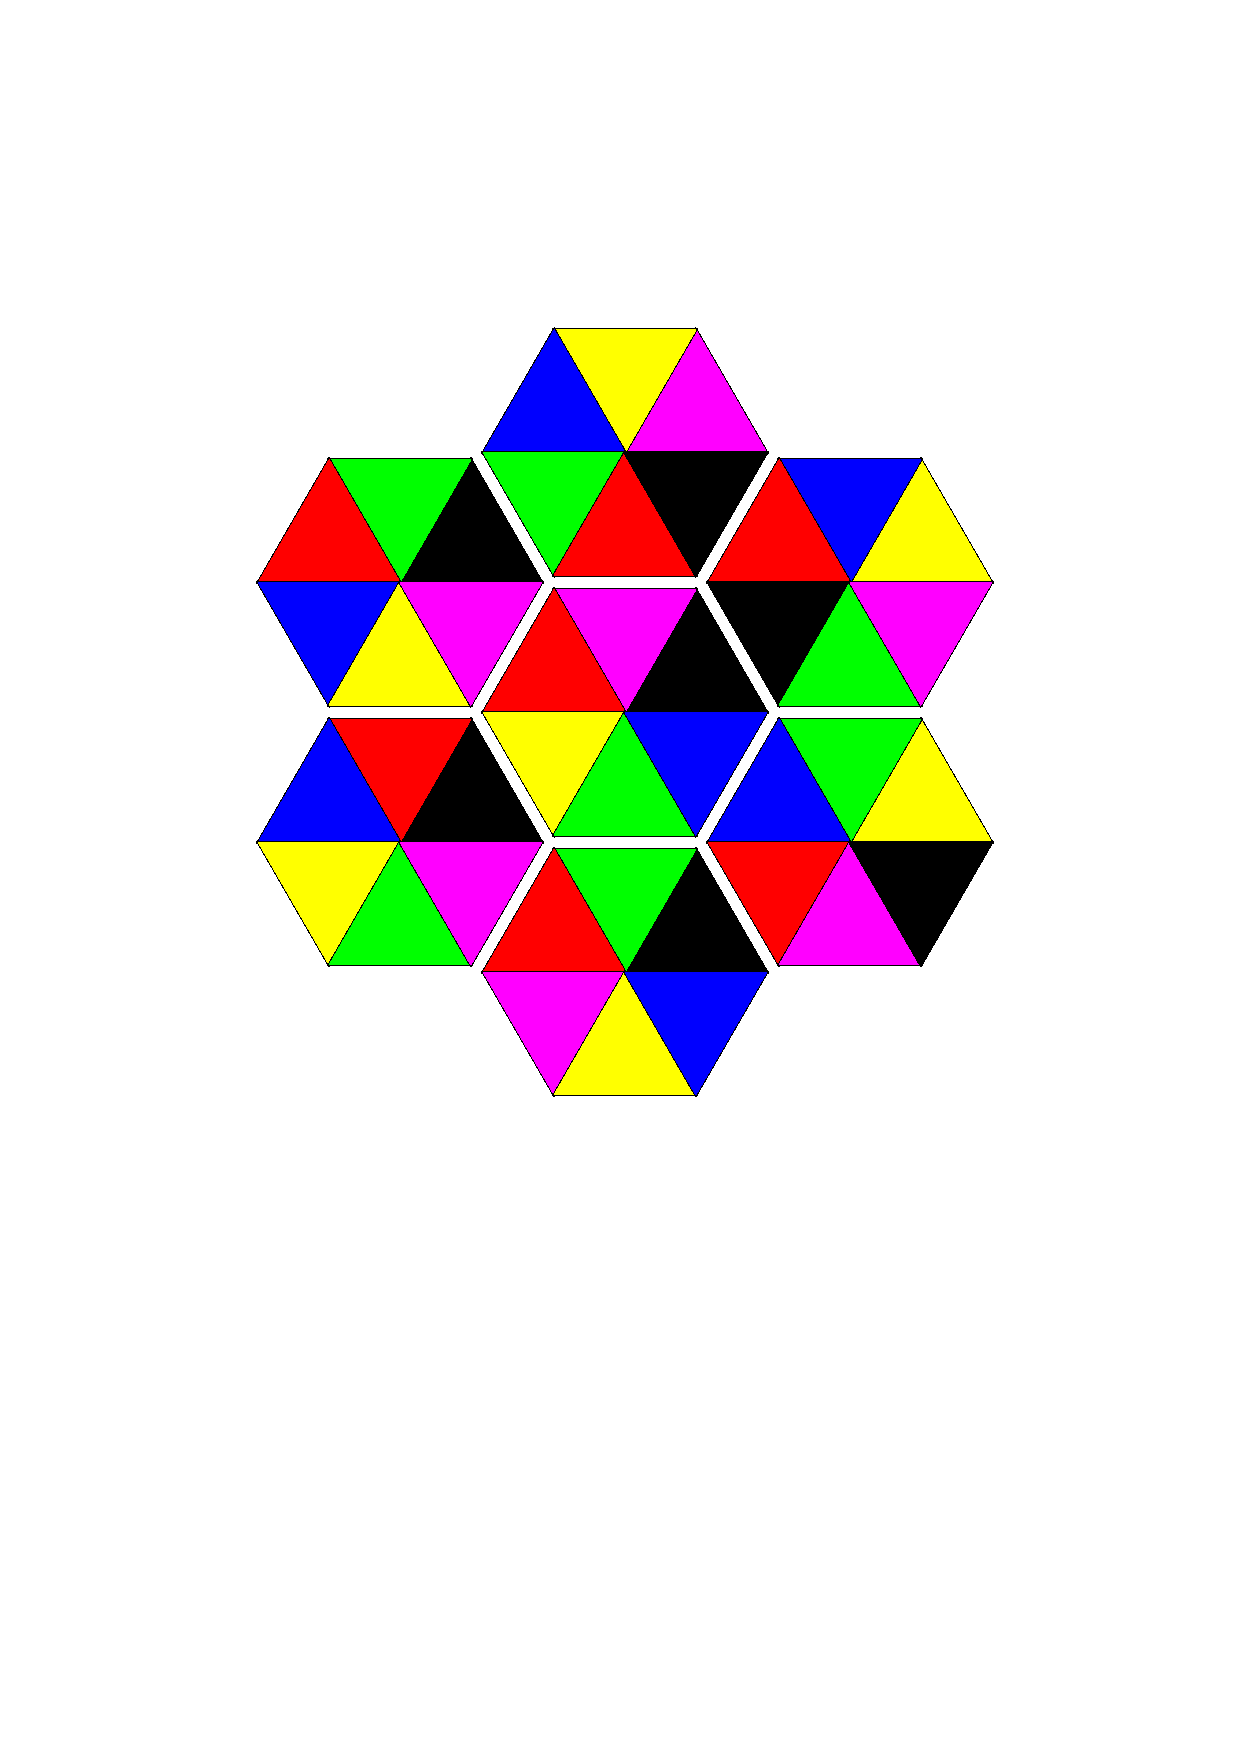
\includegraphics[width=.8\textwidth]{images/hexagons.pdf}
\end{center}

Ahhoz, hogy megoldjuk ezt a feladatot, először
valahogy le kell írnunk az ismert tényeket -- tehát
itt azt, hogy milyen lapok léteznek. A lapok színeit
egy \pr{l} struktúrába fogjuk össze, és a következő
tényeket kapjuk:
\begin{program}
lap(l(fekete,lila,sárga,kék,zöld,piros)).
lap(l(fekete,zöld,piros,kék,sárga,lila)).
lap(l(fekete,zöld,lila,sárga,kék,piros)).
lap(l(fekete,lila,piros,sárga,zöld,kék)).
lap(l(fekete,piros,kék,sárga,zöld,lila)).
lap(l(fekete,sárga,zöld,kék,piros,lila)).
lap(l(fekete,zöld,piros,lila,sárga,kék)).
\end{program}

Így például végig tudunk menni a lapokon a
\begin{query}
?- lap(L).
\end{query}
kérdés segítségével.

A lapok tetszőlegesen elforgathatóak, tehát a forgatásukra is kell valami mód. Ehhez először egyezzünk meg abban, hogy pontosan milyen elhelyezést jelent a színeknek egy sorrendje:
\begin{center}
  
\includegraphics[width=.3\textwidth]{images/hexagon.pdf}
\end{center}

Tehát az első szín van délnyugatra, a második délre,
\dots a hatodik északnyugatra. Egy forgatás során
annyi történik, hogy valamelyik másik szín kerül
előre, de utána a sorrend változatlan. Ezt így
írhatjuk le:
\begin{program}
forgat(l(A,B,C,D,E,F), l(A,B,C,D,E,F)).
forgat(l(A,B,C,D,E,F), l(B,C,D,E,F,A)).
forgat(l(A,B,C,D,E,F), l(C,D,E,F,A,B)).
forgat(l(A,B,C,D,E,F), l(D,E,F,A,B,C)).
forgat(l(A,B,C,D,E,F), l(E,F,A,B,C,D)).
forgat(l(A,B,C,D,E,F), l(F,A,B,C,D,E)).
\end{program}

A következő feladat, hogy arra adjunk egy szabályt,
hogy mikor kapcsolódik helyesen két lap. Ehhez azt
is kell tudni, hogy egymáshoz képest hogyan
helyezkednek el. A \pr{kapcsolódik(L1, L2, Irány,
  F1, F2)} azt mondja, hogy ha az \pr{L1} laptól
\pr{Irány} irányba helyezzük le az \pr{L2} lapot,
akkor a két lap elforgatható egy \pr{F1} illetve
\pr{F2} helyzetbe úgy, hogy a találkozásuknál a
színek megegyeznek. Itt az irány leírására
használhatnánk a fent bevezetett számokat, de jobban
olvasható talán, ha égtájakat használunk. Nézzük meg
először a \pr{dny} (délnyugat) irányt!
\begin{program}
kapcsolódik(L1, L2, dny, F1, F2) :-
    forgat(L1, F1), forgat(L2, F2),
    F1 = l(X,_,_,_,_,_),
    F2 = l(_,_,_,X,_,_).
\end{program}
A törzs első sora csak annyit mond, hogy az \pr{F1}
és \pr{F2} az \pr{L1} és \pr{L2} elforgatottja; a
második és harmadik sor pedig azt biztosítja, hogy
az elforgatott lapokon a \emph{megfelelő} helyen
levő szín megegyezik (a többi nem számít). Mivel az
\pr{L1}-től délnyugatra van az \pr{L2}, ezért az
\pr{L1} délnyugati (első) színe az érdekes, az
\pr{L2}-nek pedig a szemben levő, tehát északkeleti
(negyedik) színe.

Teljesen hasonlóan felírhatjuk a többi égtájra is a
kapcsolódási szabályokat:
\begin{program}
kapcsolódik(L1, L2, d, F1, F2) :-
    forgat(L1, F1), forgat(L2, F2),
    F1 = l(_,X,_,_,_,_),
    F2 = l(_,_,_,_,X,_).
kapcsolódik(L1, L2, dk, F1, F2) :-
    forgat(L1, F1), forgat(L2, F2),
    F1 = l(_,_,X,_,_,_),
    F2 = l(_,_,_,_,_,X).
kapcsolódik(L1, L2, ék, F1, F2) :-
    forgat(L1, F1), forgat(L2, F2),
    F1 = l(_,_,_,X,_,_),
    F2 = l(X,_,_,_,_,_).
kapcsolódik(L1, L2, é, F1, F2) :-
    forgat(L1, F1), forgat(L2, F2),
    F1 = l(_,_,_,_,X,_),
    F2 = l(_,X,_,_,_,_).
kapcsolódik(L1, L2, ény, F1, F2) :-
    forgat(L1, F1), forgat(L2, F2),
    F1 = l(_,_,_,_,_,X),
    F2 = l(_,_,X,_,_,_).
\end{program}

Most már minden megvan ahhoz, hogy megkeressük a
megoldást. Ezt úgy találjuk meg, hogy veszünk 7
különböző (!) lapot, és felírjuk a rájuk vonatkozó
kapcsolódási feltételeket:
\begin{program}
megoldás(F1, F2, F3, F4, F5, F6, F7) :-
    lap(L1),
    lap(L2), L2 \= L1,
    lap(L3), L3 \= L1, L3 \= L2,
    lap(L4), L4 \= L1, L4 \= L2, L4 \= L3,
    lap(L5), L5 \= L1, L5 \= L2, L5 \= L3, L5 \= L4,
    lap(L6), L6 \= L1, L6 \= L2, L6 \= L3, L6 \= L4,
             L6 \= L5,
    lap(L7), L7 \= L1, L7 \= L2, L7 \= L3, L7 \= L4,
             L7 \= L5, L7 \= L6,
    kapcsolódik(L1, L2, dk,  F1, F2),
    kapcsolódik(F1, L7, ék,  F1, F7),
    kapcsolódik(F2, L3, ék,  F2, F3),
    kapcsolódik(F2, F7, é,   F2, F7),
    kapcsolódik(F3, L4, é,   F3, F4),
    kapcsolódik(F3, F7, ény, F3, F7),
    kapcsolódik(F4, L5, ény, F4, F5),
    kapcsolódik(F4, F7, dny, F4, F7),
    kapcsolódik(F5, L6, dny, F5, F6),
    kapcsolódik(F5, F7, d,   F5, F7),
    kapcsolódik(F6, F1, d,   F6, F1),
    kapcsolódik(F6, F7, dk,  F6, F7).
\end{program}
Itt a lapok számozása szintén a fenti módon
történik, a 7-es számú a középső lap. Az első hét
sor csak felveszi a lapokat, és biztosítja, hogy
mindegyik különböző legyen. Utána jönnek a szabályok
-- itt egy dologra kell figyelni, hogy (a
procedurális olvasat értelmében) a \pr{kapcsolódik}
szabályok kielégítése sorrendben történik, ezért
amint egy lapot ,,letettünk'', annak meghatározódik
a forgatása, tehát onnantól kezdve a forgatás
nélküli \pr{L} helyett az elforgatott \pr{F}-et kell
használni. Ezzel megköveteljük, hogy a
\pr{kapcsolódik}ban a ,,sima'' és ,,elforgatott''
változat megegyezzen, tehát ne tudja tovább forgatni
a lapot.

Keressük meg akkor a megoldást!
\begin{query}
?- megoldás(F1, F2, F3, F4, F5, F6, F7).
F1 = l(kék, zöld, piros, fekete, lila, sárga),
F2 = l(kék, sárga, lila, fekete, zöld, piros),
F3 = l(fekete, piros, kék, sárga, zöld, lila),
F4 = l(sárga, zöld, kék, piros, lila, fekete),
F5 = l(sárga, kék, fekete, zöld, piros, lila),
F6 = l(fekete, lila, piros, sárga, zöld, kék),
F7 = l(fekete, zöld, lila, sárga, kék, piros)
\end{query}

Ebben a programban rengeteg az ismétlés, ami nem túl
szép, de a jelenlegi eszközeinkből ennyire
futja. Nemsokára megismerkedünk a listákkal és a
számolással, amelyek segítségével a \pr{forgat} és a
\pr{kapcsolódik} szabályokat egy--egy sorban meg
lehetne oldani, és a \emph{megoldás}ban a lapok
különbözőségét is könnyebben lehetne biztosítani.

\chapter{Listák}
\section{Listák}
Blabla
\section{Projekt: Dobble Kids}
Blabla

% -*- fill-column: 52 -*-
% (local-set-key (kbd "C-c C-f") 'display-fill-column-indicator-mode)
\chapter{Operátorok}
Van még szintaktikus cukor bizonyos struktúrákon:
ezek az \emph{operátorok}. Amikor például leírunk
egy olyan matematikai kifejezést, hogy $2a+bc$, vagy
a szorzásokat csillaggal (\pr{*}) jelölve,
\pr{2*a+b*c}, akkor a szorzás és összeadás műveletek
az argumentumaik \emph{között} szerepelnek. Ezeket
hívjuk \emph{infix} (,,közbülső'') operátoroknak. Ha
egy ilyen kifejezést a szokásos \emph{prefix}
(,,elülső'') funktorokkal szeretnénk leírni, akkor
ezt kapnánk:
\index{operátor}
\index{operátor!prefix}
\index{operátor!infix}
\begin{query}
+(*(2, a), *(b, c))
\end{query}
Vannak nyelvek, amelyek ezt preferálják, és vannak
olyanok, amelyek a \emph{posztfix} (,,hátulsó'')
operátorokat:
\index{operátor!posztfix}
\begin{query}
((2, a)*, (b, c)*)+
\end{query}
... de a Prolog ezekre a megszokott infix
jelöléseket támogatja.

\begin{infobox*}{}{pre-, in- és posztfix}
Kizárólag prefix operátorokkal működnek a
\emph{Lisp} nyelvcsalád nyelvei (Common Lisp,
Scheme, Clojure, Racket etc.) Ezeknél a funktor neve
is a zárójelen belülre kerül, tehát a fenti példából
ez lesz: {\tt (+ (* 2 a) (* b c))}
\index{Lisp}

Ennek az egyik előnye a következetesség, a másik
pedig, hogy a műveletek kiterjeszthetőek több
argumentumra. Lispben például értelmes a {\tt (+ 1 2
  3 4 5)} kifejezés, amelynek értéke 15.

Kizárólag posztfix operátorokkal működnek a
\emph{veremnyelvek}, mint pl.~a Forth vagy a
PostScript. Itt minden operátornak csak egyféle
aritása lehet, de cserébe megszabadulunk a
zárójelektől. A fenti példa Forthban: {\tt 2 a * b c
  * +} \index{Forth}\index{veremnyelv}

Ezt hívják \emph{Reverse Polish Notation}-nek (RPN,
,,fordított lengyel jelölés''). Sok számológép is
használja; elsőre elég furcsa, de nagyon kényelmes és gyors,
ha megszokjuk.
\index{RPN}
\end{infobox*}

Tetszőleges funktorból lehet operátort csinálni. Az
egyargumentumú funktorok lehetnek pre- vagy
posztfixek, a kétargumentumúak pedig csak
infixek. Ahhoz, hogy egy ilyen kifejezést értelmezni
lehessen, még azt is kell tudni, hogy melyik operátornak
van elsőbbsége -- például a szorzást előbb kell
elvégezni, mint az összeadást, tehát elsőbbsége van.
\index{elsőbbség}

A Prologban az ilyen jellegű ,,beállításokat'' olyan
szabályokkal lehet megadni, amelyeknek nincsen feje,
csak törzse. Néhány példa operátorok definíciójára
(ezek részei az alapbeállításnak):
\begin{program}
:- op(200, fy, -).
:- op(400, yfx, *).
:- op(500, yfx, +).
:- op(1000, xfy, ',').
:- op(1200, xfx, :-).
\end{program}
Itt az első, 1 és 1200 közti szám adja meg a
\emph{precedenciá}\/t (minél kisebb, annál korábban
kell elvégezni az adott műveletet), a második a
típusát, és a harmadik magát az operátort.
\index{precedencia}

Hétféle típus létezik:
\begin{itemize}
\item \pr{xfx}, \pr{xfy}, \pr{yfx}: infix operátorok
\item \pr{fx}, \pr{fy}: prefix operátorok
\item \pr{xf}, \pr{yf}: posztfix operátorok
\end{itemize}

Ezeket úgy kell értelmezni, hogy az \pr{f} mutatja
az operátor helyét, az \pr{x} és \pr{y} pedig az
argumentumo(ka)t. Ha egy argumentum \pr{x}-el van
jelölve, akkor -- amennyiben az is egy operátoros
kifejezés -- az \pr{x} operátorának szigorúan kisebb
precedenciájúnak kell lennie az \pr{f}-nél. Ezzel
szemben az \pr{y} esetében ez nem csak kisebb lehet,
hanem egyenlő is. A zárójelezés minden előtt
elsőbbséget élvez (0 a precedenciája).

Nézzünk ez alapján egy pár példát arra, hogy a
Prolog különböző kifejezéseket hogyan elemez:
\begin{enumerate}
\item Mivel a \pr{+} operátor \pr{yfx} típusú, ha
  egy \pr{a + b + c} kifejezésem van, akkor ezt nem
  értelmezhetem úgy, hogy \pr{+(a, +(b, c))}, mert
  akkor a külső \pr{+} második argumentumában levő
  \pr{+(b, c)} kifejezés precedenciája megegyezik a
  \pr{+}-éval (hiszen az is \pr{+}). Viszont ha
  \pr{+(+(a, b), c)} módon értelmezem, ez a probléma
  nem lép fel: az első argumentumban levő \pr{+(a,
    b)} kifejezés precedenciája ugyan ugyanaz, de ez
  megengedett, mert a baloldali egy
  \pr{y}-argumentum. Tehát az \pr{yfx} operátorokat
  {\bf balról jobbra} kell zárójelezni.
\item A \pr{-a * (b + c * d)} kiértékelését először
  a zárójeles rész-szel kell kezdeni. Ezt nem
  értelmezhetem úgy, hogy \pr{*(+(b, c), d)}, mivel
  a \pr{+} precedenciája nagyobb a \pr{*}-énál, az
  \pr{yfx} szerint pedig kisebbnek vagy egyenlőnek
  kéne lennie. Ezért a helyes értelmezés a \pr{+(b,
    *(c, d))}. Ezután jön a 200-as precedenciájú
  1-argumentumú \pr{-} operátor, és végül a 400-as
  precedenciájú \pr{*}. A teljes kifejezés tehát így
  néz ki: \pr{*(-(a),+(b,*(c,d)))}.
\item A \pr{P :- Q, R, S} kifejezés helyes
  zárójelezése \pr{:-(P, ','(Q, ','(R, S)))}, mivel
  az \pr{xfy} típusú vessző operátort {\bf jobbról
  balra} kell zárójelezni, és a \pr{:-} operátor
  precedenciája a legmagasabb.
\item Mivel a \pr{:-} operátor \pr{xfx} típusú,
  ezért {\bf nem szerepelhet a saját
  argumentumaként}. Egy olyan kifejezésnek, hogy
  \pr{a :- b :- c}, nincsen helyes zárójelezése.
\item A negálás \pr{fy} típusú, ezért a \pr{- -a}
  kifejezés is elfogadható (a két mínuszjelet el
  kell választani, különben egy \pr{-{}-} nevű
  operátor lesz belőle); ha \pr{fx} típusú lenne,
  akkor ezt zárójelezni kéne \pr{-(-a)} alakban.
\end{enumerate}
A precedencia tehát többek közt azt is meghatározza,
hogy mi egy kifejezésben az elsődleges funktor,
ezért pl.
\begin{query}
?- X+Y = 2*3+5.
X = 2*3
Y = 5
?- X*Y = 2*3+5.
false
\end{query}

Nem csak különleges karakterekkel megadott
funktorokból készíthetünk operátorokat, hanem
tetszőleges nevűekből. Ez magyarul kevésbé
természetes, mint angolul, de azért nézzünk erre is
példát!
\begin{query}
:- op(600, xfx, benne_van).
X benne_van L :- tartalmaz(X, L).
\end{query}
Ez definiálja a \pr{tartalmaz} funktor infix
változatát. Ezután
\begin{query}
?- b benne_van [a, b, c].
true
?- benne_van(b, [a, b, c]).
true
\end{query}

\begin{infobox}{}{izoláló nyelvek}
A magyar nyelv ragozási rendszere mellett egy-egy
operátorrá tett szó magában még nem képes
természetes mondatok készítésére, de más nyelvekben
ez nagyon jól működik. Ezek az ún.~\emph{izoláló}
nyelvek -- jellemzően ilyenek a (dél)kelet-ázsiai
nyelvek, pl. kínai, indonéz vagy thai, de bizonyos
mértékig az angol is.
\end{infobox}

\begin{problem}
Mit ad az alábbi program:
\begin{query}
t(0+1, 1+0).
t(X+0+1, X+1+0).
t(X+1+1, Z) :- t(X+1, X1), t(X1+1, Z).
\end{query}
\dots a következő kérdésekre:
\begin{query}
?- t(0+1, A).
?- t(0+1+1, B).
?- t(1+0+1+1+1, C).
?- t(D, 1+1+1+0).
\end{query}
\end{problem}

\section{Számolás}
Ahogy az előző feladatban is látszott, a matematikai
kifejezések a Prolog számára csak struktúrák, és
ezért az
\begin{query}
?- X = 1 + 2.
\end{query}
kérdésre azt a (nem túl sokatmondó) választ kapjuk,
hogy
\begin{query}
X = 1 + 2
\end{query}

Ha rá akarjuk kényszeríteni, hogy kiértékelje a
kifejezést, az egyenlőség helyett az \pr{is}
operátort használhatjuk:
\begin{query}
?- X is 1 + 2.
X = 3
\end{query}

A matematikai kifejezésekben használható az
összeadás (\pr{+}), kivonás/negáció (\pr{-}),
szorzás (\pr{*}), osztás (\pr{/}), egészosztás
(\pr{//}), hatványozás (\pr{**}), és a
maradékszámítás (\pr{mod}). Néhány példa:
\begin{query}
?- X is 5/2.
X = 2.5
?- X is 9//2.
X = 4 % 9-ben 4-szer van meg (teljesen) a 2
?- X is 2**128.
X = 340282366920938463463374607431768211456.
?- X is 10 mod 3.
X = 1 % 10-nek a 3-mal vett osztási maradéka 1
\end{query}
\index{\pr{+}}\index{\pr{*}}\index{\pr{**}}
\index{\pr{-}}\index{\pr{/}}\index{\pr{//}}
\index{\pr{mod}}

Szintén alkalmazhatóak olyan gyakran használt
matematikai függvények, mint az abszolutérték
(\pr{abs}), a szinusz (\pr{sin}), vagy a természetes
alapú logaritmus (\pr{log}).
\index{\pr{abs}}\index{\pr{sin}}\index{\pr{log}}

A relációs jelek szintén ,,kiértékelő erővel''
bírnak, tehát pl.
\begin{query}
?- 2 + 2 > 3.
true
\end{query}
A nagyobb-egyenlő és kisebb-egyenlő relációk rendre
\pr{>=} és \pr{=<}, a matematikai egyenlőség és
különbözőség pedig \pr{=:=} és \pr{=\textbackslash=}, pl.
\index{\pr{>}}\index{\pr{<}}
\index{\pr{>=}}\index{\pr{=<}}
\index{\pr{=:=}}\index{\pr{=\textbackslash=}}
\begin{query}
?- 2 + 3 = 6 - 1.
false
?- 2 + 3 =:= 6 - 1.
true
?- 2 + 3 \= 6 - 1.
true
?- 2 + 3 =\= 6 - 1.
false
\end{query}

A matematikai kiértékelésnél feltétel, hogy a
kifejezésben ne szerepeljen változó. Tehát a
rendszer nem tudja azt megválaszolni, hogy:
\begin{query}
?- X + 2 < X + 3.
\end{query}
\dots bármennyire is nyilvánvalónak tűnik nekünk.

Az \pr{is} és az \pr{=:=} időnként ugyan
felcserélhető, de általában nem:
\begin{query}
X is 1 + 2.  % OK, X = 3
X =:= 1 + 2. % Nem jó, nem lehet benne ismeretlen
3 is 1 + 2.  % OK, baloldalt lehet szám
3 =:= 1 + 2. % OK
1 + 2 is 3.  % Nem jó, baloldalt nem lehet kifejezés
1 + 2 =:= 3. % OK
\end{query}

\subsection*{Legnagyobb közös osztó}

Két szám legnagyobb közös osztójának megkeresése
klasszikus probléma. Az alábbi megoldás ötlete
Euklidész \emph{Elemek} c. művéből származik
(i.e.~300 körül).
\index{algoritmus!euklidészi}

Legyen \pr{lnko(N, M, O)} igaz, ha \pr{N} és \pr{M}
legnagyobb közös osztója \pr{O}. Ha a két szám
azonos, akkor az osztó is az lesz:
\index{\pr{lnko}}
\begin{program}
lnko(N, N, N).
\end{program}
Ha az első szám a kisebb, akkor azt levonhatjuk a
másodikból, és a legnagyobb közös osztó nem
változik:
\begin{program}
lnko(N, M, O) :-
    N < M,
    M1 is M - N,
    lnko(N, M1, O).
\end{program}
Végül, ha a második szám a kisebb, akkor egyszerűen
cseréljük meg a két számot, és az előző esethez
jutunk:
\begin{program}
lnko(N, M, O) :-
    N > M,
    lnko(M, N, O).
\end{program}
Könnyen látszik, hogy a 3.~típusú lépés után mindig
2.~típusú jön, és a 2.~típusú lépés után az \pr{N +
  M} összeg csökken. Mivel a számok nem mehetnek 0
alá, előbb-utóbb biztosan eljut az 1.~típusú
lépéshez, ahol megkapjuk az eredményt.

Teszteljük!
\begin{query}
?- lnko(1071, 462, X).
X = 21.
\end{query}

A fenti magyarázatok deklaratív jellegűek. A
procedurális olvasata a programnak a következő:
\begin{enumerate}
\item Ha \pr{N = M}, akkor a legnagyobb közös osztó
  \pr{N}. Vége.
\item Ha \pr{N < M}, akkor vonjuk ki \pr{M}-ből
  \pr{N}-et, és menjünk vissza az 1.~lépésre.
\item Ha \pr{N > M}, akkor cseréljük meg \pr{N}-et
  és \pr{M}-et, és menjünk vissza az 1.~lépésre.
\end{enumerate}
Az ilyen megoldási módszereket \emph{algoritmusnak}
nevezik.\index{algoritmus}

\begin{infobox}{}{algoritmusok}
Bár Euklidész algoritmusa régi, de már sokkal
régebben is léteztek hasonló módszerek, pl.~az ókori
Mezopotámiában a sumérok már i.e.~2500 körül
ismertek algoritmust az osztásra. Maga az elnevezés
egy Bagdadban tanító VIII--IX.~századi perzsa
matematikus nevéből származik, akit (arabosan) úgy
hívtak, hogy Muhammad bin Múszá \emph{al-Khvárizmí}
(,,a Hvárezmből való Mózes fia Mohamed'').
\index{al-Khvárizmí}

Ha már a kezdeteknél tartunk, az első program, amelyet
tényleg számítógépre írtak, Ada Lovelace (1815--1852)
nevéhez fűződik, aki Byronnak, a híres költőnek
a lánya volt. A program a Bernoulli-számokat számította
ki; a gép pedig, amire írta, egy mechanikus
számítógép volt, a \emph{Difference Engine}. Ezt
Charles Babbage (1791--1871) tervezte, de csak
születésének 200 éves évfordulájára készült el
(viszont működött!).
\index{Ada Lovelace}\index{Babbage}
\end{infobox}

\subsection*{Listák hossza}
Most, hogy már tudunk számolni, ki tudjuk számítani
egy lista hosszát is:
\begin{program}
hossz([], 0).
hossz([_|M], N) :- hossz(M, N1), N is 1 + N1.
\end{program}
Egy üres lista hossza 0, egyébként meg a maradék
hossza plusz egy.
\index{\pr{hossz}}

Ha a fenti definícióban az \pr{is} helyett \pr{=}-t
használunk, akkor látjuk, hogyan számol:
\begin{query}
?- hossz([a,b,c], X).
X = 1+(1+(1+0))
\end{query}

Egy másik lehetőség, hogy egy középső argumentumban
számon tartjuk az eddigi hosszt:
\begin{program}
hossz2([], N, N).
hossz2([_|M], C, N) :- C1 is 1 + C, hossz2(M, C1, N).
hossz2(L, N) :- hossz2(L, 0, N).
\end{program}
Itt a \pr{hossz2(L1, C, N)}-re mindig igaz lesz,
hogy a teljes lista hossza az az \pr{L1} lista
hossza + \pr{C}-vel egyenlő.

A lényeges különbséget a \pr{trace} mutatja:
\begin{query}
?- trace, hossz([a, b, c], X).
Call: hossz([a, b, c], X)
  Call: hossz([b, c], X1)
    Call: hossz([c], X2)
      Call: hossz([], X3)
      Exit: hossz([], 0)
      Call: X2 is 1+0
      Exit: 1 is 1+0
    Exit: hossz([c], 1)
    Call: X1 is 1+1
    Exit: 2 is 1+1
  Exit: hossz([b, c], 2)
  Call: X is 1+2
  Exit: 3 is 1+2
Exit: hossz([a, b, c], 3)
X = 3

?- trace, hossz2([a, b, c], X).
Call: hossz2([a, b, c], X)
  Call: hossz2([a, b, c], 0, X)
    Call: C1 is 0+1
    Exit: 1 is 0+1
    Call: hossz2([b, c], 1, X)
      Call: C2 is 1+1
      Exit: 2 is 1+1
      Call: hossz2([c], 2, X)
        Call: C3 is 2+1
        Exit: 3 is 2+1
        Call: hossz2([], 3, X)
        Exit: hossz2([], 3, 3)
      Exit: hossz2([c], 2, 3)
    Exit: hossz2([b, c], 1, 3)
  Exit: hossz2([a, b, c], 0, 3)
Exit: hossz2([a, b, c], 3)
X = 3
\end{query}
Az első verzióban, miután elértünk az üres listáig,
még hozzá kell adogatnunk az 1-eket a hosszhoz. A
második verzióban viszont ilyenkor már nincs más
feladatunk, csak visszatérni a már kiszámolt
eredménnyel. Ez utóbbit úgy hívják, hogy
,,vég-rekurzió'', mivel a szabálynak a legvégén van
a rekurziós lépés. Az algoritmusok ilyen felírása
gyakran hatékonyabb, ahogy azt mindjárt látni
fogjuk.

\subsection*{Fibonacci-számok}
A Fibonacci-számokat úgy képezzük, hogy elkezdjük
két 1-essel, és utána mindig az előző két szám
összegét vesszük:
\begin{query}
1 1 2 3 5 8 13 21 34 55 ...
\end{query}
Számoljuk ki az $n$-edik Fibonacci-számot!
\begin{program}
fib(1, 1).
fib(2, 1).
fib(N, M) :-
    N1 is N - 1, N2 is N - 2,
    fib(N1, K1), fib(N2, K2),
    M is K1 + K2.
\end{program}

Próbáljuk ki!
\begin{query}
?- fib(10, X).
X = 55
?- fib(20, X).
X = 6765
\end{query}
Működik, de nagyobb számokra (pl.~40) már nem tudja
kiszámolni. A problémát az okozza, hogy a kisebb
Fibonacci-számokat feleslegesen újra és újra,
rengetegszer kiszámolja.

Próbáljuk ezt is vég-rekurzióval megoldani! Két
plusz argumentumként vegyük fel az ,,előző'' két
számot (\pr{K1} és \pr{K2}):
\begin{program}
fib2(1, M, _, M).
fib2(N, K1, K2, M) :-
    N1 is N - 1, K3 is K1 + K2,
    fib2(N1, K2, K3, M).
fib2(N, M) :- fib2(N, 1, 1, M).
\end{program}
Nézzük meg, mit csinál! Először beállítja \pr{K1}-et
és \pr{K2}-t 1-re, majd minden lépésben (i)
csökkenti az \pr{N}-et, (ii) a \pr{K1} helyére rakja
a \pr{K2}-et, és (iii) a \pr{K2} helyére rakja a
(régi) \pr{K1} és \pr{K2} összegét. Ez alapján
könnyen belátható, hogy a \pr{fib2(I, K1, K2, M)}-re
mindig igaz lesz, hogy az \pr{N-I+1}-edik Fibonacci
szám a \pr{K1} lesz (\pr{I = N} esetén világos;
a második szabály pedig nem rontja el).

Így már nagy értékekre is jól működik, hiszen minden
Fibo\-nacci-számot csak egyszer számol ki.

\begin{problem}
\item Írj szabályt, amivel két szám közül ki
lehet választani a nagyobbat!
\begin{query}
?- max(2, 5, X).
X = 5
\end{query}
\end{problem}
\begin{problem}
\item Írj szabályt, amivel egy listából ki lehet
választani a legnagyobb elemet!
\begin{query}
?- maximum([5, 2, 8, 3], X).
X = 8
\end{query}
\end{problem}
\begin{problem}
\item Írj szabályt, amivel ki lehet számolni egy
listában levő számok összegét!
\begin{query}
?- összeg([5, 2, 8, 3], X).
X = 18
\end{query}
\end{problem}
\begin{problem}
\item Írj szabályt, ami eldönti, hogy egy lista
elemei növekvő sorrendben vannak-e!
\begin{query}
?- növekvő([2, 5, 6, 8]).
true
?- növekvő([2, 6, 5, 8]).
false
\end{query}
\end{problem}
\begin{problem}
\item Írj szabályt, amivel egy listából ki lehet
választani elemeket úgy, hogy az összegük egy
adott szám legyen!
\begin{query}
?- részösszeg([1, 2, 5, 3, 2], 5, X).
X = [1, 2, 2]
X = [2, 3]
X = [5]
...
\end{query}
\end{problem}
\begin{problem}
\item Írj egy \pr{között(N1, N2, X)} szabályt,
ami eldönti, hogy az \pr{X} az \pr{N1} és az
\pr{N2} között van-e (a határokat beleértve)!
\begin{query}
?- között(2, 5, 3).
true
?- között(2, 5, 5).
true
?- között(2, 5, X).
X = 2
X = 3
...
\end{query}
\end{problem}
\begin{problem}
\item Készíts \pr{ha}, \pr{akkor},
\pr{egyébként} és \pr{:=} operátorokat, hogy
lehessen ilyeneket írni:
\begin{query}
ha X > Y akkor Z := A egyébként Z := B
\end{query}
Ennek hatására a \pr{Z} egyesül a \pr{A}-val vagy \pr{B}-vel
attól függően, hogy \pr{X} nagyobb-e, mint \pr{Y}. Például:
\begin{query}
?- X = 2, Y = 3,
   X2 is 2 * X, X4 is 4 * X,
   ha Y > X2 akkor Z := Y egyébként Z := X4,
   ha Z > 5 akkor W := 1 egyébként W := 0.
X = 2
Y = 3
Z = 8
W = 1
X2 = 4
X4 = 8
\end{query}

Prefix jelölésben ugyanez így nézne ki:
\begin{query}
ha(akkor(>(X, Y), egyébként(:=(Z, A), :=(Z, B))))
\end{query}
A szabály maga tehát nagyon egyszerű:
\begin{program}
ha(akkor(>(X, Y), egyébként(:=(Z, V), _))) :-
    X > Y, Z = V.
ha(akkor(>(X, Y), egyébként(_, :=(Z, V)))) :-
    X =< Y, Z = V.
\end{program}
Itt érdemes megjegyezni, hogy a baloldalon szereplő
\pr{>} operátornak nincsen semmilyen matematikai
értelme, csak egy struktúra funktoraként szerepel.

A feladat tehát az, hogy állítsd be úgy az
operátorokat, hogy a fenti példa működjön.
\end{problem}

\section{Projekt: Kígyó-kocka}

\begin{center}
\includegraphics[width=.6\textwidth]{images/snake-cube.jpg}
\end{center}

Oldjuk meg a jól ismert ,,kígyó-kocka'' feladványt!
Az egyes kis szakaszok fixek, de a derékszögű
fordulásoknál egymáson elforgathatóak; a feladat,
hogy kirakjunk belőle egy 3x3-as kockát.

Szokás szerint azzal kezdjük, hogy felvesszük az
adatokat. Ez a készítendő kocka mérete, és a kígyót
alkotó szakaszok hosszai:
\begin{program}
méret(3).
kígyó([3,2,2,3,2,3,2,2,3,3,2,2,2,3,3,3,3]).
\end{program}

A teljes kockán belül minden pozíciót 3
koordinátával tudunk jellemezni:
\begin{program}
pozíció(p(X, Y, Z)) :-
    méret(N), között(1, N, X),
    között(1, N, Y), között(1, N, Z).
\end{program}
Tehát a jelenlegi $3\times3$-as kocka esetében minden
koordináta 1 és 3 között változhat.

A \pr{között} szabály feladatként szerepelt,
így definiálhatjuk:
\begin{program}
között(N, M, N) :- N =< M.
között(N, M, X) :-
    N < M, N1 is N + 1,
    között(N1, M, X).
\end{program}
\index{\pr{között}}
Itt arra érdemes figyelni, hogy \pr{N > M} esetén ez
nem kielégíthető.

Hatféle irányról beszélhetünk, a három tengely
irányában pozitív és negatív irányban. Ezeket
leírhatjuk olyan módon, mint pl. \pr{i(x, -1)} vagy
\pr{i(z, 1)}. Az összes irányt tehát így
fogalmazhatjuk meg:
\begin{program}
irány(i(T,I)) :-
    tartalmaz(T, [x,y,z]),
    tartalmaz(I, [-1,1]).
\end{program}
A \pr{T} itt az egyik tengely, az \pr{I} pedig 1
vagy -1, ami a pozitív ill. negatív irányt jelöli.

Két egymás után következő szakasz mindig merőleges
egymásra, tehát a \emph{tengelyük} nem lehet azonos:
\begin{program}
köv_irány(i(T,_), i(T1,I)) :-
    irány(i(T1,I)), T \= T1.
\end{program}

Hogyan változik egy pozíció, ha ellépünk egy adott
irányban? A \pr{lépés(P1, I, P2)} akkor lesz igaz,
amikor a \pr{P1}-ből \pr{I} irányba ellépve a
\pr{P2}-be jutunk:
\begin{program}
lépés(p(X,Y,Z), i(x,I), p(X1,Y,Z)) :- X1 is X + I.
lépés(p(X,Y,Z), i(y,I), p(X,Y1,Z)) :- Y1 is Y + I.
lépés(p(X,Y,Z), i(z,I), p(X,Y,Z1)) :- Z1 is Z + I.
\end{program}
(Ezért volt jó a pozitív/negatív irányt 1-el és
-1-el jelölni.)

Próbáljuk meg felírni a megoldást! Legyen erre a
szabályunk \pr{megoldás(K, PL, I, X)}; itt \pr{K} a
kígyó hátralevő része, \pr{PL} a már kitöltött
pozíciók listája (az elején a kígyó feje, amit épp
vizsgálunk), az \pr{I} az aktuális irány, és \pr{X}
az irányváltoztatások listája. A reláció akkor
teljesül, ha a \pr{PL} pozíció-lista első elemétől
\pr{I} irányban indulva le tudjuk rakni a \pr{K}
listában levő szakaszokat az \pr{X} listában levő
irányokat követve úgy, hogy mindig a kockán belül
maradunk, és nem megyünk bele a \pr{PL} egyik
elemébe sem. Ekkor a
\begin{query}
?- kígyó(K), pozíció(P), irány(I),
   megoldás(K, [P], I, X).
\end{query}
kérdésre \pr{P} adja a kezdő pozíciót, \pr{I} a
kezdő irányt, és \pr{X} az irányváltoztatásokat.

Ha a kígyónak már csak 1 szakasza van hátra, akkor
csak azt kell megnézni, hogy azt le tudjuk-e tenni:
\begin{program}
megoldás([N], PL, I, [I]) :- ellenőriz(PL, I, N, _).
\end{program}
Az \pr{ellenőriz(PL, I, N, PL1)} akkor lesz igaz, ha
a \pr{PL} elején levő pozícióról az \pr{I} irányban
le tudunk helyezni egy \pr{N} hosszú szakaszt
anélkül, hogy kimennénk a kockából vagy érintenénk
egy \pr{PL}-ben levő pozíciót, és az így bővült
pozíció-lista a \pr{PL1}.

Ezt szavakban elmondani bonyolultabb, mint
programban:
\begin{program}
ellenőriz(PL, _, 1, PL).
ellenőriz([P|M], I, N, PL1) :-
    N > 1, lépés(P, I, P1),
    pozíció(P1), nemtartalmaz(P1, M), N1 is N - 1,
    ellenőriz([P1, P|M], I, N1, PL1).
\end{program}
Ha a szakasz 1 kockából áll, akkor nincs további
teendőnk, és \pr{PL1 = PL}. Egyébként teszünk a
megadott irányban egy lépést, megnézzük, hogy
érvényes pozíció-e, nem szerepel-e az eddigi
pozíciók listájában, és ha ez mind jó, akkor jöhet a
többi lépés -- ehhez a \pr{PL}-et kiegészítjük az új
\pr{P1} pozícióval, és a készítendő szakasz hosszát
csökkentjük 1-el.

Ha a kígyó több szakaszból áll, akkor először
ellépünk az első szakasz hosszával az aktuális
irányban, utána új irányt választunk, és rekurzióval
elvégezzük a maradékot:
\begin{program}
megoldás([N|M], PL, I, [I|X]) :-
    ellenőriz(PL, I, N, PL1), köv_irány(I, I1), 
    megoldás(M, PL1, I1, X).
\end{program}

Ezzel a fent ismertetett módon megkapjuk a
megoldást, de kicsit nehezen olvasható
alakban. Fordítsuk le magyarra az irányokat!
\begin{program}
fordít([], []).
fordít([i(T, I)|M], [F|FM]) :-
    (  T = x, (I = 1, F = jobbra; I = -1, F = balra)
     ; T = y, (I = 1, F = fel;    I = -1, F = le)
     ; T = z, (I = 1, F = előre;  I = -1, F = hátra)
    ), 
    fordít(M, FM).
\end{program}
A \pr{fordít} szabály első argumentuma irányok egy
listája, a második pedig az ennek megfelelő
fordítások listája. Érdemes megfigyelni a
zárójelezés és a logikai vagy jelentésű
pontosvesszők használatát.

Végül akkor tegyük az egész megoldót egy szabályba!
\begin{program}
kígyó_kocka(K, P, FI, FX) :-
    kígyó(K), pozíció(P), irány(I),
    megoldás(K, [P], I, X), fordít([I|X], [FI|FX]).
\end{program}

Ha kipróbáljuk:
\begin{query}
?- kígyó_kocka(K, P, FI, FX).
FI = jobbra,
FX = [jobbra, fel, balra, előre, fel, hátra, jobbra,
      előre, le, balra, fel, hátra, fel, előre, le,
      jobbra, fel],
K = [3, 2, 2, 3, 2, 3, 2, 2, 3, 3, 2, 2, 2, 3, 3, 3,
     3],
P = p(1, 1, 1)
\end{query}
... az eredmény már sokkal könnyebben értelmezhető.

A megoldó elég általános ahhoz, hogy más
változatokra is használható legyen, pl. a ,,mean
green'' feladványra, ha lecseréljük a \pr{kígyó}
definícióját:
\begin{program}
kígyó([3,3,2,3,2,3,2,2,2,3,3,3,2,3,3,3]).
\end{program}
Egy másik variáns a ,,king'' feladvány, amelynél
$4\times4$-es kockát kell építeni:
\begin{program}
méret(4).
kígyó([3,2,3,2,2,4,2,3,2,3,2,3,2,2,2,2,
       2,2,2,2,3,3,2,2,2,2,2,3,4,2,2,2,
       4,2,3,2,2,2,2,2,2,2,2,2,4,2]).
\end{program}
Ennek sokkal több lehetőséget kell megvizsgálnia,
ezért kell neki pár perc.

Megfordíthatjuk a kérdést: hogyan lehet egy
számsorozatot készíteni, ami olyan kígyót határoz
meg, amelyből kocka készíthető? Ehhez a \pr{kígyó}-nak
egy új definíciójára lesz szükségünk:
\begin{program}
kígyó(K) :-
    méret(N), N3 is N^3, N1 is N3 // (N - 1),
    között(N1, N3, H), hossz(K, H),
    kígyó(K, N3).
\end{program}
A teljes kígyó hossza a méret köbe (\pr{N3}). A
kígyót alkotó szakaszok száma (a kígyónak, mint
szakasz-listának a \emph{hossza}, \pr{H}) tehát
\pr{N3/(N-1)} és \pr{N3} között lesz, hiszen minden
szakasz legfeljebb \pr{N-1} új pozíciót fedhet
le. Az egyes szakaszokat ezután a \pr{kígyó/2}
segítségével készítjük el:
\begin{program}
kígyó([], 1).
kígyó([Sz|K], M) :-
    M > 1, méret(N), között(2, N, Sz),
    M1 is M - Sz + 1, kígyó(K, M1).
\end{program}
Ha még \pr{M} hosszú kígyót kell csinálni, akkor
választunk egy számot 2 és \pr{N} között (egy
szakasz hossza csak ilyen lehet), ez lesz a mostani
szakaszunk hossza, és a maradék szakaszokkal pedig
egy ennyivel rövdebb kígyót csinálunk (pontosabban
eggyel hosszabbat, mert egy szakasz utolsó eleme
egyben a következő első eleme). Amikor már csak 1
hosszú kígyót kell csinálni, készen vagyunk.

Ezzel a definícióval azt kapjuk, hogy
\begin{query}
?- kígyó_kocka(K, P, FI, FX).
K = [2, 3, 3, 2, 3, 3, 3, 3, 3, 3, 3, 2, 3, 2, 3],
P = p(1, 2, 2),
FI = le,
FX = [le, jobbra, fel, hátra, le, balra, fel, előre,
      le, jobbra, fel, balra, hátra, le, előre] 
\end{query}
(Ez jó sokáig tart.) Mivel a szakaszok számával
alulról felfele próbálkozunk, az első megoldás a
legkevesebb szakaszból álló kígyó (15 db), amit
$3\times3$-as kockába lehet rendezni. Ha a fenti
definícióban a \pr{között(N1, N3, H)} helyett \pr{H
  = 15}-öt írunk (tehát ha lerögzítjük a szegmensek
számát), akkor gyorsan lefut.

A futási idő mindig egy kompromisszum: (aránylag)
keveset kellett gondolkodnunk ahhoz, hogy megírjuk
ezt a programot. Hatékonyabb programot gyakran
nehezebb írni, viszont néha elég a lassabb is,
pl.~olyan feladatoknál, mint a kígyó-generálás,
amikor a lényeg csak az, hogy találjunk egy
megoldást (még ha akár napokig is kell a gépnek
számolnia). Azért persze törekedjünk a
hatékonyságra!

\subsection*{A teljes program}

Mivel ez már egy elég összetett program volt, itt
van egyben az egész:

\begin{program}
tartalmaz(X, [X|_]).
tartalmaz(X, [_|M]) :- tartalmaz(X, M).

nemtartalmaz(_, []).
nemtartalmaz(X, [Y|M]) :- X \= Y, nemtartalmaz(X, M).

hossz([], 0).
hossz([_|M], N) :- hossz(M, N1), N is 1 + N1.

között(N, M, N) :- N =< M.
között(N, M, X) :-
    N < M, N1 is N + 1,
    között(N1, M, X).

% Standard
méret(3).
kígyó([3,2,2,3,2,3,2,2,3,3,2,2,2,3,3,3,3]).

% Mean green
% méret(3).
% kígyó([3,3,2,3,2,3,2,2,2,3,3,3,2,3,3,3]).

% King
% méret(4).
% kígyó([3,2,3,2,2,4,2,3,2,3,2,3,2,2,2,2,
%        2,2,2,2,3,3,2,2,2,2,2,3,4,2,2,2,
%        4,2,3,2,2,2,2,2,2,2,2,2,4,2]).

% Generáló
% méret(3).
% kígyó(K) :-
%     méret(N), N3 is N^3, N1 is N3 // (N - 1),
%     között(N1, N3, H), hossz(K, H),
%     kígyó(K, N3).
% kígyó([], 1).
% kígyó([Sz|K], M) :-
%     M > 1, méret(N), között(2, N, Sz),
%     M1 is M - Sz + 1, kígyó(K, M1).

pozíció(p(X, Y, Z)) :-
    méret(N), között(1, N, X),
    között(1, N, Y), között(1, N, Z).

irány(i(T,I)) :-
    tartalmaz(T, [x,y,z]),
    tartalmaz(I, [-1,1]).

köv_irány(i(T,_), i(T1,I)) :-
    irány(i(T1,I)), T \= T1.

lépés(p(X,Y,Z), i(x,I), p(X1,Y,Z)) :- X1 is X + I.
lépés(p(X,Y,Z), i(y,I), p(X,Y1,Z)) :- Y1 is Y + I.
lépés(p(X,Y,Z), i(z,I), p(X,Y,Z1)) :- Z1 is Z + I.

ellenőriz(PL, _, 1, PL).
ellenőriz([P|M], I, N, PL1) :-
    N > 1, lépés(P, I, P1),
    pozíció(P1), nemtartalmaz(P1, M), N1 is N - 1,
    ellenőriz([P1, P|M], I, N1, PL1).

megoldás([N], PL, I, [I]) :- ellenőriz(PL, I, N, _).
megoldás([N|M], PL, I, [I|X]) :-
    ellenőriz(PL, I, N, PL1), köv_irány(I, I1), 
    megoldás(M, PL1, I1, X).

fordít([], []).
fordít([i(T, I)|M], [F|FM]) :-
    (  T = x, (I = 1, F = jobbra; I = -1, F = balra)
     ; T = y, (I = 1, F = fel;    I = -1, F = le)
     ; T = z, (I = 1, F = előre;  I = -1, F = hátra)
    ), 
    fordít(M, FM).

kígyó_kocka(K, P, FI, FX) :-
    kígyó(K), pozíció(P), irány(I),
    megoldás(K, [P], I, X), fordít([I|X], [FI|FX]).
\end{program}

% -*- fill-column: 52 -*-
% (local-set-key (kbd "C-c C-f") 'display-fill-column-indicator-mode)
\chapter{Vezérlés}
\section{Rendezések}
Egy klasszikus -- és nagyon hasznos -- programozási
feladat számok listájának növekvő sorrendbe
rendezése. Erre rengeteg módszer van, itt csak a
legfontosabbak közül nézünk meg néhányat.

\subsection*{Beszúrásos rendezés}
Az első algoritmus a \emph{beszúrásos rendezés}. Az
ötlet a következő: ha van egy listám, akkor azt
szétszedem az első elemre és a maradékára, az
utóbbit (rekurzívan) rendezem, és végül az első
elemet beszúrom a ,,megfelelő'' helyre.
\index{rendezés!beszúrásos}
\begin{program}
rendez1([], []).
rendez1([X|M], Y) :-
    rendez1(M, M1), beszúr(X, M1, Y).
\end{program}
A megfelelő helyre való beszúrásnál pedig egyszerűen
addig megyünk, amíg egy legalább akkora elemet nem
találunk:
\begin{program}
beszúr(X, [], [X]).
beszúr(X, [Y|M], [X,Y|M]) :- X =< Y.
beszúr(X, [Y|M], [Y|M1]) :- X > Y, beszúr(X, M, M1).
\end{program}
Próbáljuk ki!
\begin{query}
?- rendez1([4,1,9,2,6,0,3,2,5,1], X).
X = [0, 1, 1, 2, 2, 3, 4, 5, 6, 9]
\end{query}

Ennek az algoritmusnak egy nagy előnye, hogy akkor
is jól használható, ha az adatokat folyamatosan
kapjuk, hiszen ha már van egy rendezett listánk,
akkor utána mindig elég a \pr{beszúr} műveletet
használni. Egy másik jó tulajdonsága, hogy egy már
rendezett sorozatnál nem végez plusz munkát, épp
csak ellenőrzi, hogy a lista tényleg jó sorrendben
van:
\begin{query}
?- trace, rendez1([1,2,3], X).
Call:rendez1([1, 2, 3], X)
  Call:rendez1([2, 3], X1)
    Call:rendez1([3], X2)
      Call:rendez1([], X3)
      Exit:rendez1([], [])
      Call:beszúr(3, [], X2)
      Exit:beszúr(3, [], [3])
    Exit:rendez1([3], [3])
    Call:beszúr(2, [3], X1)
      Call:2=<3
      Exit:2=<3
    Exit:beszúr(2, [3], [2, 3])
  Exit:rendez1([2, 3], [2, 3])
  Call:beszúr(1, [2, 3], X)
    Call:1=<2
    Exit:1=<2
  Exit:beszúr(1, [2, 3], [1, 2, 3])
Exit:rendez1([1, 2, 3], [1, 2, 3])
X = [1, 2, 3]
\end{query}

Ugyanakkor ha nincs szerencsénk, nem túl jó
hatásfokú: ha a lista $n$ hosszú, akkor kb.~$n^2$
összehasonlítást végez a legrosszabb esetben.

\subsection*{Gyorsrendezés}
A gyorsrendezésnél kiválasztunk egy tetszőleges
elemet (pl.~az elsőt), és a többit két részre
osztjuk aszerint, hogy nagyobb-e ennél vagy
sem. Ezután a két részt külön--külön rendezzük
(rekurzívan), majd az eredmény ezek összefűzéséből
adódik:
\index{rendezés!gyors}
\begin{program}
rendez2([], []).
rendez2([X|M], Y) :-
    szétoszt(X, M, Kicsi, Nagy),
    rendez2(Kicsi, K),
    rendez2(Nagy, N),
    hozzáfűz(K, [X|N], Y).
\end{program}
A szétosztás elég magától értetődő:
\begin{program}
szétoszt(_, [], [], []).
szétoszt(X, [Y|M], K, [Y|N]) :-
    X =< Y, szétoszt(X, M, K, N).
szétoszt(X, [Y|M], [Y|K], N) :-
    X > Y, szétoszt(X, M, K, N).
\end{program}

Ez (nagyon hosszú listákra) bizonyíthatóan sokkal
kevesebb ellenőrzést végez, mint a beszúrásos
rendezés. A fenti program azonban a hozzáfűzések
miatt nem igazán hatékony -- a következő leckében
majd szó lesz a különbség-listákról, amelyek
segítségével sokkal gyorsabbá tehető.

\subsection*{Fésülő rendezés}
Utolsónak nézzünk meg egy nagyon hasonló
algoritmust: itt is két részre bontjuk mindig a
listát, azokat rendezzük, majd összefűzzük, de itt
nem a szétválasztás a bonyolultabb, hanem az
összefűzés, vagy ez esetben az \emph{összefésülés}.
\index{rendezés!fésülő}

A listát a felénél kettéosztjuk, és mindkét részt
rendezzük (rekurzívan), végül a két rendezett listát
egy listává fésüljük össze:
\begin{program}
rendez3([], []).
rendez3([X], [X]).
rendez3(X, Y) :-
    kettéoszt(X, X1, X2),
    rendez3(X1, Y1),
    rendez3(X2, Y2),
    összefésül(Y1, Y2, Y).

kettéoszt([], [], []).
kettéoszt([X], [X], []).
kettéoszt([X,Y|M], [X|M1], [Y|M2]) :-
    kettéoszt(M, M1, M2).
\end{program}

Az összefésülésnél a két lista elemét
összehasonlítjuk, és a megfelelőt berakjuk a
maradékok összefűzéséből kapott listába:
\begin{program}
összefésül([X|Mx], [Y|My], [X|M]) :-
    X =< Y, összefésül(Mx, [Y|My], M).
összefésül([X|Mx], [Y|My], [Y|M]) :-
    X > Y, összefésül([X|Mx], My, M).
összefésül(X, [], X).
összefésül([], Y, Y).
\end{program}

Itt érdekes módon azt tapasztaljuk, hogy a (helyes)
eredményt végtelen sokszor megkapjuk. Ez azért van,
mert a \pr{rendez3} harmadik szabálya az egyelemű
listákra is meghívódhat. Ezt ki lehetne védeni
azzal, hogy megköveteljük, hogy legyen legalább két
eleme:
\begin{program}
rendez3(X, Y) :-
    X = [_,_|_], Y = [_,_|_],
    kettéoszt(X, X1, X2),
    rendez3(X1, Y1),
    rendez3(X2, Y2),
    összefésül(Y1, Y2, Y).
\end{program}
\dots de ez nem a legelegánsabb. (Hasonlóan, az
\pr{összefésül} utolsó két szabálya közt is van
átfedés.) Nincs valami jobb mód erre?

\begin{infobox*}{}{furcsa rendezések}
Rendezési algoritmusokból nincs hiány. Bizonyítható,
hogy a gyorsrendezés, a fésülő rendezés (és még sok
másik) a lehető leghatékonyabb\dots kivéve egy-két
furcsa módszert:
\begin{enumerate}
\item Vágjunk (száraz) spagettitésztákat az egyes
  számoknak megfelelő hosszokra, majd marokra fogva
  tegyük le az asztalra. Ezután egy kartonlapot
  rátéve mindig sorban vegyük ki azt, ami hozzáér a
  laphoz, és így egy csökkenő sorrendezéshez jutunk.
\item Vegyük a lista egy véletlenszerű
  permutációját, és ellenőrizzük, hogy sorban
  van-e. Ha igen, készen vagyunk. Ha nem, akkor
  robbantsuk fel a világot. Feltéve, hogy igaz a
  párhuzamos univerzumok elmélete, csak az az
  univerzum fog megmaradni, amelyikben a véletlen
  permutáció pont a helyes sorbarendezés volt.
\end{enumerate}
\index{rendezés!spagetti}\index{rendezés!véletlen}
\end{infobox*}      

\section{Vágás}
Egy szabály törzsében \emph{vágást} eszközölhetünk a
\pr{!} segítségével. Ez azt mondja, hogy ha már
idáig eljutottunk, akkor vagy sikerül teljesíteni a
törzs maradék részét, vagy ha nem, akkor úgy
vesszük, hogy ezzel a fejjel való egyesítés
sikertelen volt, nem próbálunk a \pr{!} előtti
kifejezésekre visszamenni, vagy az azonos fejhez
tartozó esetleges többi szabályt megnézni.
\index{vagas@vágás}\index{\pr{"!}}

Nézzük meg például az alábbi szabályokat, ahol
\pr{A}, \pr{B}, \pr{C} stb. kifejezéseket jelölnek:
\begin{program}
C :- P, Q, R, !, S, T, U.
C :- V.

A :- B, C, D.
\end{program}

Ekkor ha az
\begin{query}
?- A.
\end{query}
kérdést feltesszük, a következő fog történni:
\begin{enumerate}
\item Megnézi, hogy \pr{B} teljesül-e (tegyük fel,
  hogy igen).
\item Megnézi, hogy \pr{P}, \pr{Q}, \pr{R}
  teljesülnek-e (tegyük fel, hogy igen).
\item Megnézi, hogy \pr{S}, \pr{T}, \pr{U}
  teljesülnek-e. Tegyük fel, hogy az \pr{S} és
  \pr{T} teljesül, de az \pr{U} nem. Ekkor szokás
  szerint visszamegy a \pr{T}-re, és megkeresi annak
  egy másik megoldását stb.
\item Ha nem sikerült az \pr{S}, \pr{T}, \pr{U}-t
  teljesíteni, akkor -- a vágás miatt -- már nem
  megy vissza, hogy az \pr{R} egy másik megoldását
  keresse, és nem próbálkozik a \pr{C}-hez tartozó
  második szabállyal sem, hanem egy szinttel feljebb
  megy, és a \pr{B}-hez keres egy másik megoldást.
\end{enumerate}

\subsection*{Összefésülés hatékonyabban}
Nézzük meg, hogyan lehet ezzel feljavítani az összefésülést!
\begin{program}
összefésül([X|Mx], [Y|My], [X|M]) :-
    X =< Y, !, összefésül(Mx, [Y|My], M).
összefésül([X|Mx], [Y|My], [Y|M]) :-
    X > Y, !, összefésül([X|Mx], My, M).
összefésül(X, [], X) :- !.
összefésül([], Y, Y) :- !.
\end{program}

A vágások a programot hatékonyabbá teszik: ha az
első szabályban láttuk, hogy \pr{X =< Y}, már nem
kell ellenőrizni a többi szabályt stb. (Az utolsó
sorban a vágás felesleges, csak a szimmetria
kedvéért került bele.)

Hasonlóan, a \pr{rendez3} második szabályában:
\begin{program}
rendez3([X], [X]) :- !.
\end{program}
Ezekkel a módosításokkal már egyértelmű
(\emph{determinisztikus}) lesz a megoldás.
\index{determinisztikusság}

A vágások nem változtatják meg a program értelmét
(tehát, hogy milyen kifejezésekre lesz igaz), csak a
hatékonyságát.

\subsection*{Maximum}
Nézzünk egy másik példát! Az alábbi szabály két szám
közül kiválasztja a nagyobbikat:
\begin{program}
max1(X, Y, X) :- X >= Y.
max1(X, Y, Y) :- X < Y.
\end{program}
A fenti módon ez átírható így:
\begin{program}
max2(X, Y, X) :- X >= Y, !.
max2(X, Y, Y) :- X < Y.
\end{program}

Felmerül azonban ekkor, hogy a második szabályban szükség
van-e egyáltalán az \pr{X < Y} összehasonlításra,
hiszen csak akkor juthatunk oda, ha az \pr{X >= Y}
nem teljesült. A program akkor is működni látszik,
ha elhagyjuk:
\begin{program}
max3(X, Y, X) :- X >= Y, !.
max3(_, Y, Y).
\end{program}

Teszteljük egy kicsit!
\begin{query}
?- max3(3, 5, X).
X = 5
?- max3(4, 2, X).
X = 4
?- max3(1, 5, 5).
true
?- max3(5, 1, 1). % Ajjaj...
true
\end{query}

Hoppá! Mi történt?  Mivel az utolsó példában
mindhárom argumentumnak van értéke, és az első és
harmadik nem azonos, az első szabállyal nem is
próbálkozik, hanem rögtön a másodikra megy, ami
pedig most, hogy kivettük a feltételt, teljesül.

A \pr{max3} változatban megváltozott a program
deklaratív jelentése, hiszen egy olyan tényt
tartalmaz, ami magában nézve nem igaz. Ez általában
kerülendő, bár a hatékonysághoz néha szükséges. Ha
ilyen gondolatmenetet alkalmazunk, nagyon óvatosnak
kell lenni -- itt pl. biztosnak kell lennünk benne,
hogy a harmadik argumentum mindig változó.

\subsection*{Hozzáadás halmazhoz}
Egy további példaként nézzük meg az alábbi szabályt:

\begin{program}
% hozzáad(+X, +Halmaz, -Eredmény).
% Hozzáadja X-et a Halmaz listához,
% de csak akkor, ha az még nem tartalmazta.
hozzáad(X, L, L) :- tartalmaz(X, L), !.
hozzáad(X, L, [X|L]).
\end{program}

A vágás nélkül itt a második szabályt nehezebb lenne
megfogalmazni, kéne hozzá a 3. leckéhez tartozó
projektben látott \pr{nemtartalmaz} szabály, és
következésképp a hatékonyságból is vesztene.

Cserébe itt is problémába ütközünk, ha a harmadik
argumentum nem változó:
\begin{query}
?- hozzáad(b, [a,b], [b,a,b]).
true
\end{query}
Ezt elkerülendő, érdemes a dokumentációval\index{dokumentáció}
egyértelművé tenni a használatot. A fenti programhoz
tartozó megjegyzés is ilyen szellemben íródott. Az
első sorában egy egyezményes jelölésrendszert
használ, melyben minden argumentum háromféle lehet:
\begin{itemize}
\item \pr{+X} : kell, hogy legyen értéke
\item \pr{?X} : lehet értéke, de nem muszáj
\item \pr{-X} : csak változó lehet
\end{itemize}
Például:
\begin{enumerate}
\item \pr{+X > +Y} [4.~lecke]
\item \pr{lapít(+Eredeti, -Lapos)} [3.~lecke]
\item \pr{tartalmaz(?Elem, ?Lista)} [3.~lecke]
\end{enumerate}
Az első esetben mindkét kifejezésnek ismertnek kell
lennie; a másodikban a lapítandó lista ismert, és a
lapított verzió csak változó lehet; a harmadikban
pedig mind a lista, mind a benne tartalmazandó elem
lehet változó vagy ismert is.

\begin{problem}
Nézzük meg az alábbi szabályokat!
\begin{program}
p(1).
p(2) :- !.
p(3).
\end{program}       
Mit lesz az összes válasz az alábbi kérdésekre:
\begin{query}
?- p(X).
?- p(X), p(Y).
?- p(X), !, p(Y).
\end{query}
\end{problem}
\begin{problem}
Írd át hatékonyabbra a \pr{szétoszt} szabályt
vágások segítségével!
\end{problem}

\section{Tagadás}
Hogyan tudjuk megfogalmazni azt, hogy ,,Csilla
szeret minden állatot, kivéve a pókokat''?
\begin{program}
szereti(csilla, X) :- pók(X), !, fail.
szereti(csilla, X) :- állat(X).
\end{program}
(Általában ilyenkor a \pr{false} helyett a
\pr{fail}-t szokás használni, de a kettő jelentése
azonos.)\index{\pr{fail}}\index{tagadás}

Próbáljuk ki!
\begin{program}
állat(tarantula).
állat(denevér).
pók(tarantula).
\end{program}
\begin{query}
?- szereti(csilla, tarantula).
false
?- szereti(csilla, denevér).
true
\end{query}
Ez annyira hasznos, hogy érdemes bevezetni, mint
tagadást:
\begin{program}
nem(P) :- P, !, fail.
nem(_).
\end{program}

Figyeljük meg, hogy itt valami olyat csináltunk,
amit eddig még soha: egy változót (\pr{P}) a
törzsben magában használtunk. Ez feltételezi, hogy a
\pr{P}-nek kiszámolható az igazságértéke. Például a
fenti példát átírva:
\begin{program}
szereti(csilla, X) :- állat(X), nem(pók(X)).
\end{program}
Itt a \pr{P} értéke a \pr{pók(X)} struktúra, és a
\pr{nem} törzsében levő \pr{P} kiértékelésekor ezt
mint megoldandó célkifejezést értelmezi.
(A szabvány szerint elvileg \pr{call(P)}-t kellene írni,\index{\pr{call}}
de a legtöbb Prolog rendszerben a \pr{P} is elegendő,
erről bővebben lesz még szó a következő fejezetben.)

\subsection*{A ,,zárt világ'' feltétel}
A tagadásnak ez a módja nem mindig intuitív. Egy így
tagadott kifejezés akkor lesz igaz, ha a kifejezés
nem bizonyítható.\index{zart@zárt világ}

Mi történik, ha az előző programban felcseréljük a
törzs két tagját?
\begin{program}
szereti(csilla, X) :- nem(pók(X)), állat(X).
\end{program}
Érdekes módon Csilla most már a denevéreket sem
szereti! Miért? Azért, mert a \pr{nem(pók(X))}-ben
az \pr{X} egy változó, tehát a \pr{pók(X)}
bizonyítható az \pr{X = tarantula} helyettesítéssel,
így a \pr{nem(pók(X))} nem teljesül. Az érték
nélküli argumentumokkal tehát vigyázni kell.

Hasonlóan furcsa lehet, hogy
\begin{query}
?- nem(állat(kutya)).
true
\end{query}
\dots de persze helyes, hiszen a programban levő
szabályok alapján nem bizonyítható, hogy a kutya
állat.

Ezek miatt a \pr{nem} (vagy az angol \pr{not})
helyett a \pr{\textbackslash+} operátort szokás
használni, melynek definíciója ugyanaz, csak az
elnevezés kevésbé félrevezető:
\begin{program}
szereti(csilla, X) :- állat(X), \+ pók(X).
\end{program}
\index{\pr{\textbackslash+}}

\begin{problem}
Milyen kérdéssel lehet a \pr{Jelöltek} listából
kiválasztani azokat, akik nem szerepelnek a
\pr{Kiesettek} listában? Használd a
\pr{tartalmaz} szabályt és a tagadást!
\end{problem}
\begin{problem}
Készíts szabályt, ami két halmaz különbségét
képzi! (A halmaz itt egy olyan lista, amelyben minden
elem egyszer fordul elő.)
\begin{query}
?- különbség([a,b,c,d], [f,d,b,e], X).
X = [a, c]
\end{query}
\end{problem}
\begin{problem}
Készíts szabályt, ami kiválogatja egy listából
azokat a kifejezéseket, amelyek egy adott másik
kifejezéssel egyesíthetőek!
\begin{query}
?- egyesíthető([X,b,t(Y)], t(a), L).
L = [X, t(Y)]
\end{query}
Figyelj arra, hogy az \pr{X} és \pr{Y} ne kapjon
ezáltal értéket!
\end{problem}

\section{Projekt: Katamino}
Készítsünk megoldót a Katamino-feladványokhoz!

\begin{center}
\includegraphics[width=.8\textwidth]{images/katamino.jpg}
\end{center}

A feladat mindig az, hogy a 12 pentominó egy adott
részhalmazából rakjunk ki egy $5\times n$-es
téglalapot.

\subsection*{Reprezentáció}
Az első lépés továbbra is az, hogy valahogyan le
kell írni a gép számára az adatokat, vagyis a
használható alakzatokat. Sokféle leírás
elképzelhető; itt most csináljuk a következőt:
minden egyes alakzatot a körülírható téglalap bal
alsó sarkához képest számolt koordinátáival írjuk
le.

Például a T-alakzatnál:
\begin{center}
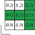
\includegraphics[width=.3\textwidth]{images/pentomino.pdf}
\end{center}
Ha a bal alsó sarok a $(0,0)$ pont, akkor az
alakzathoz tartozó pontok a következők: $(0,1)$,
$(1,1)$, $(2,0)$, $(2,1)$ és $(2,2)$. A pontokat
$x$-koordináta szerint, és azon belül $y$-koordináta
szerint rendezve írjuk fel.

Az $x$ és $y$-koordináták összefogására bármilyen
struktúrát használhatunk, pl. \pr{p(0,1)}, de a
tömörség kedvéért szokás a \pr{-} operátort
alkalmazni: \pr{0-1}. Bár az egyes
forgatások/tükrözések programból is legenerálhatóak,
egyszerűbb mindegyiket külön adatként megadni.

A T esetében pl.:
\begin{program}
alakzat(t, [0-0,0-1,0-2,1-1,2-1]).
alakzat(t, [0-0,1-0,1-1,1-2,2-0]).
alakzat(t, [0-1,1-1,2-0,2-1,2-2]).
alakzat(t, [0-2,1-0,1-1,1-2,2-2]).
\end{program}

Hasonlóan lehet definiálni a többi alakzatot,
amelyek mind valamilyen 1 betűből álló kódot kaptak:
\pr{k}, \pr{p}, \pr{c} stb. (Az összes alakzat, a
teljes program forráskódjával együtt, a lecke végén
található.)

\subsection*{Megoldó}
A programunk fő szabálya a \pr{kirak} lesz, ami egy
alakzat-listához megadja, hogy hogyan fog kinézni a
tábla. A megoldás módszere nagyon egyszerű: mindig a
(balról/alulról) első lyukat próbáljuk betömni.

\begin{program}
kirak(Ak, X) :- hossz(Ak, N), kirak(Ak, N, [], X).

kirak([], _, T, T).
kirak(Ak, N, T, X) :-
    első_lyuk(N, T, P),
    töröl(A, Ak, Ak1),
    letesz(A, P, N, T, T1),
    kirak(Ak1, N, T1, X).
\end{program}
A 2-argumentumú változat megnézi, hogy hány
alakzatot kapott (tehát milyen hosszú a tábla), és
meghívja a 4-argumentumú testvérét. Ez a
felhasználható alakzatokon (\pr{Ak}) kívül még
megkapja a tábla hosszát (\pr{N}), a tábla jelenlegi
állapotát (\pr{T}), és ezáltal kiszámolja a
kitöltött táblát (\pr{X}).

Ehhez megkeresi az első lyukat, majd kiválaszt
(töröl) egy alakzatot, azt leteszi úgy, hogy lefedje
a lyukat, és rekurzívan folytatja a műveletet, amíg
mindent le nem rak.

A tábla állapotát egy listában tároljuk, amelynek az
elemei \pr{h(X-Y,A)} alakban adják meg, hogy az
\pr{X-Y} pozíción az \pr{A} alakzat egy darabja
található. Az első lyuk megkeresése így nagyon
egyszerű:
\begin{program}
első_lyuk(N, T, X-Y) :-
    között(1, N, X), között(1, 5, Y),
    \+ tartalmaz(h(X-Y,_), T), !.
\end{program}

Ez deklaratív
olvasatban azt mondja, hogy az \pr{X-Y} koordináták
a megfelelő keretek között vannak, és a tábla ezen a
pozíción nem tartalmaz elemet. Mitől fogja ez az
elsőt adni? Azért, mert a procedurális olvasatból
tudjuk, hogy sorban fog próbálkozni, tehát először
az \pr{X = 1} eseteket próbálja végig különböző
\pr{Y} értékekre, aztán az \pr{X = 2}-t stb., és a
végén levő vágásnak köszönhetően nem fog további
lyukakat megadni akkor sem, ha a keresés visszalépne
ide.

Már csak a \pr{letesz(A, X-Y, N, T, T1)} szabály van
hátra. Ez megpróbálja az \pr{A} alakzatot lerakni
úgy, hogy lefedje az \pr{X-Y} pontot, ne menjen ki
az $5\times n$-es táblából, és ne takarjon olyan
pozíciókat, amelyek szerepelnek \pr{T}-ben. Ha
sikerül, akkor az alakzat lehelyezésével kapott új
tábla a \pr{T1}.
\begin{program}
letesz(A, X-Y, N, T, T1) :-
    alakzat(A, [_-Dy|Dk]),
    Y1 is Y - Dy, Y1 > 0,
    letesz(A, X-Y1, Dk, N, [h(X-Y,A)|T], T1).
\end{program}
Ez tehát az \pr{A} alakzatnak kiválasztja egy
forgatását, és megnézi az első pontjának az
$y$-koordinátáját (\pr{Dy}). Az \pr{Y} koordinátánál
ennyivel lejjebb kell rakni az alakzatot, hogy az
első pont fedje a lyukat (hiszen az első pont az
alakzat legbaloldalibb, és azon belül legalsó
pontja). Ha ez a módosult \pr{Y1} koordináta nem
pozitív, akkor az alakzat kilóg.

A tényleges lerakási kísérletet a \pr{letesz}
6-argumentumú változata végzi:
\begin{program}
letesz(_, _, [], _, T, T).
letesz(A, X-Y, [Dx-Dy|Dk], N, T, T1) :-
    X1 is X + Dx, között(1, N, X1),
    Y1 is Y + Dy, között(1, 5, Y1),
    \+ tartalmaz(h(X1-Y1,_), T),
    letesz(A, X-Y, Dk, N, [h(X1-Y1,A)|T], T1).
\end{program}
Ez plusz argumentumként megkapja a kiválasztott
forgatáshoz tartozó pontokat is (az első kivételével,
amellyel a lyukat fedtük), és ezeken megy végig
rekurzívan. Minden lépésben a (módosított) \pr{X-Y}
koordináta alapján kiszámolja, hogy hova kerül a
pont, és ellenőrzi, hogy értelmes-e a koordináta és
nincs-e már lefedve \pr{T}-ben.

\subsection*{Kiíratás}
A lényeggel ugyan már készen vagyunk, de az eredmény
nehezen olvasható:
\begin{query}
?- kirak([l,t,w,k,y,r,z,c,p], X).
  X = [h(9-5, c), h(9-4, c), h(9-3, c), h(8-5, c),
       h(8-3, c), h(9-2, p), h(9-1, p), h(8-2, p),
       h(8-1, p), h(7-1, p), h(8-4, z), h(7-4, z),
       h(7-3, z), h(7-2, z), h(6-2, z), h(7-5, r),
       h(6-5, r), h(6-4, r), h(6-3, r), h(5-4, r),
       h(5-5, w), h(4-5, w), h(4-4, w), h(3-4, w),
       h(3-3, w), h(6-1, y), h(5-2, y), h(5-1, y),
       h(4-1, y), h(3-1, y), h(5-3, k), h(4-3, k),
       h(4-2, k), h(3-2, k), h(2-2, k), h(3-5, t),
       h(2-5, t), h(2-4, t), h(2-3, t), h(1-5, t), 
       h(2-1, l), h(1-4, l), h(1-3, l), h(1-2, l),
       h(1-1, l)]
\end{query}

Próbáljuk meg kiíratni egy kicsit ,,grafikusabb''
formában! Az elsődleges szabályunk akkor ez lesz:
\begin{program}
katamino(Ak) :-
    hossz(Ak, N), kirak(Ak, X), kiír(N, X).
\end{program}

A \pr{kiír(N, T)} pedig 5 sorba rendezve szépen
kiírja az \pr{N} hosszú \pr{T} táblát. A kiíráshoz a
\pr{write(X)} kifejezést fogjuk használni, ami
kiírja az \pr{X} értékét, új sor nyitásához pedig a
\pr{nl}-t (\emph{newline}, újsor).
\index{\pr{write}}\index{\pr{nl}}
\begin{program}
kiír(N, T) :- kiír(N, 1-5, T).

kiír(_, _-0, _).
kiír(N, X-Y, T) :-
    Y =< 5, X > N, Y1 is Y - 1,
    nl, kiír(N, 1-Y1, T).
kiír(N, X-Y, T) :-
    Y =< 5, X =< N,
    tartalmaz(h(X-Y,A), T),
    write(A), write(' '),
    X1 is X + 1,
    kiír(N, X1-Y, T).
\end{program}
A 2-argumentumú változat csak átadja a feladatot a
3-ar\-gu\-men\-tu\-mú\-nak, ami megkapja az éppen kiírandó
elem \pr{X-Y} koordinátáját is. Ennek három szabálya
van:
\begin{enumerate}
\item Ha már a 0. sort kéne kiírni, készen vagyunk.
\item Ha \pr{X > N}, akkor vége az aktuális sornak,
  új sort kezdünk. Az \pr{Y} koordináta felülről
  megy lefelé, mert a kiírás is felülről lefelé
  történik.
\item Egyébként megkeresi, hogy az \pr{X-Y} pozíción
  melyik alakzat található, és kiírja, utána kiír
  még egy szóközt, és továbbmegy a következő \pr{X}
  pozícióra.
\end{enumerate}
Nézzük meg!
\begin{query}
?- katamino([l,t,w,k,y,r,z,c,p]).
t t t w w r r c c 
l t w w r r z z c 
l t w k k r z c c 
l k k k y z z p p 
l l y y y y p p p 
true
\end{query}
És ez éppen az a megoldás, ami a képen van! Erre
persze elég jó esély volt, ugyanis a felhasználandó
alakzatok listáját hozzávetőlegesen a képen látható
megoldás sorrendjében adtuk meg. Egy másik
permutáció más megoldást talál meg először:
\begin{query}
?- katamino([t,w,l,k,r,z,y,p,c]).
w y y y y l l l l 
w w y p p p r r l 
t w w p p z z r r 
t t t k k z c r c 
t k k k z z c c c 
true 
\end{query}

\begin{problem}
A Katamino szabályai szerint a kirakandó téglalap
magassága mindig 5. Oldjuk fel ezt a korlátot!
Írd át a programot úgy, hogy a \pr{katamino}
szabály paraméterben kapja meg a magasságot is, és
ennek megfelelő megoldást keressen! A program vegye
észre rögtön, ha a magasság nem illik a megkapott
alakzatok számához (pl.~10 alakzat és 7-es
magasság). Keress megoldást a $3\times20$,
$4\times15$, $5\times12$, $6\times10$ téglalapok
kitöltésére! (Tipp: a szabályokban az eddigi \pr{N}
paramétert cseréld \pr{N-M} párra.)
\end{problem}

\subsection*{A teljes program}
\begin{program}
katamino(Ak) :-
    hossz(Ak, N), kirak(Ak, X), kiír(N, X).

% Megoldó

kirak(Ak, X) :- hossz(Ak, N), kirak(Ak, N, [], X).

kirak([], _, T, T).
kirak(Ak, N, T, X) :-
    első_lyuk(N, T, P),
    töröl(A, Ak, Ak1),
    letesz(A, P, N, T, T1),
    kirak(Ak1, N, T1, X).

első_lyuk(N, T, X-Y) :-
    között(1, N, X), között(1, 5, Y),
    \+ tartalmaz(h(X-Y,_), T), !.

letesz(A, X-Y, N, T, T1) :-
    alakzat(A, [_-Dy|Dk]),
    Y1 is Y - Dy, Y1 > 0,
    letesz(A, X-Y1, Dk, N, [h(X-Y,A)|T], T1).

letesz(_, _, [], _, T, T).
letesz(A, X-Y, [Dx-Dy|Dk], N, T, T1) :-
    X1 is X + Dx, között(1, N, X1),
    Y1 is Y + Dy, között(1, 5, Y1),
    \+ tartalmaz(h(X1-Y1,_), T),
    letesz(A, X-Y, Dk, N, [h(X1-Y1,A)|T], T1).

% Kiírás

kiír(N, T) :- kiír(N, 1-5, T).

kiír(_, _-0, _).
kiír(N, X-Y, T) :-
    Y =< 5, X > N, Y1 is Y - 1,
    nl, kiír(N, 1-Y1, T).
kiír(N, X-Y, T) :-
    Y =< 5, X =< N,
    tartalmaz(h(X-Y,A), T),
    write(A), write(' '),
    X1 is X + 1,
    kiír(N, X1-Y, T).

% Segéd-szabályok

tartalmaz(X, [X|_]).
tartalmaz(X, [_|Maradék]) :- tartalmaz(X, Maradék).

töröl(X, [X|M], M).
töröl(X, [Y|M], [Y|M1]) :- töröl(X, M, M1).

hossz([], 0).
hossz([_|M], N) :- hossz(M, N1), N is 1 + N1.

között(N, M, N) :- N =< M.
között(N, M, X) :-
    N < M, N1 is N + 1,
    között(N1, M, X).

% Alakzatok

% kígyó (lila)
alakzat(k, [0-0,0-1,0-2,1-2,1-3]).
alakzat(k, [0-0,0-1,1-1,1-2,1-3]).
alakzat(k, [0-0,1-0,1-1,2-1,3-1]).
alakzat(k, [0-0,1-0,2-0,2-1,3-1]).
alakzat(k, [0-1,0-2,0-3,1-0,1-1]).
alakzat(k, [0-1,1-0,1-1,2-0,3-0]).
alakzat(k, [0-1,1-1,2-0,2-1,3-0]).
alakzat(k, [0-2,0-3,1-0,1-1,1-2]).
% P-betű (rózsaszín)
alakzat(p, [0-0,0-1,0-2,1-0,1-1]).
alakzat(p, [0-0,0-1,0-2,1-1,1-2]).
alakzat(p, [0-0,0-1,1-0,1-1,1-2]).
alakzat(p, [0-0,0-1,1-0,1-1,2-0]).
alakzat(p, [0-0,0-1,1-0,1-1,2-1]).
alakzat(p, [0-0,1-0,1-1,2-0,2-1]).
alakzat(p, [0-1,0-2,1-0,1-1,1-2]).
alakzat(p, [0-1,1-0,1-1,2-0,2-1]).
% C-betű (sárga)
alakzat(c, [0-0,0-1,0-2,1-0,1-2]).
alakzat(c, [0-0,0-1,1-0,2-0,2-1]).
alakzat(c, [0-0,0-1,1-1,2-0,2-1]).
alakzat(c, [0-0,0-2,1-0,1-1,1-2]).
% W-betű (világoszöld)
alakzat(w, [0-0,0-1,1-1,1-2,2-2]).
alakzat(w, [0-0,1-0,1-1,2-1,2-2]).
alakzat(w, [0-1,0-2,1-0,1-1,2-0]).
alakzat(w, [0-2,1-1,1-2,2-0,2-1]).
% L-betű (narancssárga)
alakzat(l, [0-0,0-1,0-2,0-3,1-0]).
alakzat(l, [0-0,0-1,0-2,0-3,1-3]).
alakzat(l, [0-0,0-1,1-0,2-0,3-0]).
alakzat(l, [0-0,0-1,1-1,2-1,3-1]).
alakzat(l, [0-0,1-0,1-1,1-2,1-3]).
alakzat(l, [0-0,1-0,2-0,3-0,3-1]).
alakzat(l, [0-1,1-1,2-1,3-0,3-1]).
alakzat(l, [0-3,1-0,1-1,1-2,1-3]).
% Y-betű vagy tengeralattjáró (barna)
alakzat(y, [0-0,0-1,0-2,0-3,1-1]).
alakzat(y, [0-0,0-1,0-2,0-3,1-2]).
alakzat(y, [0-0,1-0,1-1,2-0,3-0]).
alakzat(y, [0-0,1-0,2-0,2-1,3-0]).
alakzat(y, [0-1,1-0,1-1,1-2,1-3]).
alakzat(y, [0-1,1-0,1-1,2-1,3-1]).
alakzat(y, [0-1,1-1,2-0,2-1,3-1]).
alakzat(y, [0-2,1-0,1-1,1-2,1-3]).
% I-betű vagy egyenes (kék)
alakzat(i, [0-0,0-1,0-2,0-3,0-4]).
alakzat(i, [0-0,1-0,2-0,3-0,4-0]).
% r-betű (szürke)
alakzat(r, [0-0,0-1,1-1,1-2,2-1]).
alakzat(r, [0-0,1-0,1-1,1-2,2-1]).
alakzat(r, [0-1,0-2,1-0,1-1,2-1]).
alakzat(r, [0-1,1-0,1-1,1-2,2-0]).
alakzat(r, [0-1,1-0,1-1,1-2,2-2]).
alakzat(r, [0-1,1-0,1-1,2-1,2-2]).
alakzat(r, [0-1,1-1,1-2,2-0,2-1]).
alakzat(r, [0-2,1-0,1-1,1-2,2-1]).
% V-betű vagy sarok (kék)
alakzat(v, [0-0,0-1,0-2,1-0,2-0]).
alakzat(v, [0-0,0-1,0-2,1-2,2-2]).
alakzat(v, [0-0,1-0,2-0,2-1,2-2]).
alakzat(v, [0-2,1-2,2-0,2-1,2-2]).
% Z-betű vagy S-betű (kék)
alakzat(z, [0-0,0-1,1-1,2-1,2-2]).
alakzat(z, [0-0,1-0,1-1,1-2,2-2]).
alakzat(z, [0-1,0-2,1-1,2-0,2-1]).
alakzat(z, [0-2,1-0,1-1,1-2,2-0]).
% pluszjel (piros)
alakzat(+, [0-1,1-0,1-1,1-2,2-1]).
% T-betű (zöld)
alakzat(t, [0-0,0-1,0-2,1-1,2-1]).
alakzat(t, [0-0,1-0,1-1,1-2,2-0]).
alakzat(t, [0-1,1-1,2-0,2-1,2-2]).
alakzat(t, [0-2,1-0,1-1,1-2,2-2]).
\end{program}

\chapter{Haladó technikák}
\section{Különbség-listák}
Blabla
\section{Struktúrák kezelése}
Blabla
\section{Magasabb rendű szabályok}
Blabla
\section{Vezérlés}
Blabla
\section{Projekt: bla}
Blabla

\chapter{Mélyvíz}
\section{Keresőfák}
Blabla
\section{Asszociációs listák}
Blabla
\section{Bináris keresőfák}
Blabla
\section{AVL-fák}
Blabla
\section{A program}
Blabla
\section{Projekt: prioritásos sor}
Blabla


\backmatter

\chapter{Könyvajánló}
Magyar nyelven nem sok minden jelent meg a Prologról, bár fontos
megemlíteni a Szeredi Péter által fejlesztett \name{Mprolog}
(\emph{Modular Prolog}) rendszerről szóló
könyvet:
\begin{itemize}[leftmargin=1.5cm,itemindent=-1cm,labelsep=0cm]
\item[] Zs.~Farkas, I.~Futó, T.~Langer, P.~Szeredi, \emph{Mprolog
programozási nyelv}, Műszaki Könyvkiadó, 1989.
\end{itemize}
Angolul már sokkal nagyobb a választék. Elsőként az Előszóban említett
két könyvet ajánlanám: az \emph{Art of Prolog} egy mélyebb,
technikaibb tárgyalása a nyelvnek, míg a Bratko-féle tankönyv számos
mesterséges intelligenciabeli alkalmazást mutat be.

A programozási készség elsajátításához a legfontosabb a gyakorlás;
rengeteg érdekes feladat található (megoldásokkal!) az alábbiakban:
\begin{itemize}[leftmargin=1.5cm,itemindent=-1cm,labelsep=0cm]
\item[] H.~Coelho, J.~C.~Cotta, \emph{Prolog by Example---How to Learn, Teach and Use It}, Springer, 1988.
\item[] B.~Demoen, Ph-L.~Nguyen, T.~Schrijvers, R.~Tron\c con, \emph{The First 10 Prolog Programming Contests}, Belgium, 2005.
\end{itemize}
Hatékony programok írásához sok hasznos és praktikus tanács-csal szolgál ez a könyv:
\begin{itemize}[leftmargin=1.5cm,itemindent=-1cm,labelsep=0cm]
\item[] R.~A.~O'Keefe, \emph{The Craft of Prolog}, MIT Press, 1990.
\end{itemize}
Végül a beépített szabályokról, fájlkezelésről és sok más hasznos
dologról egy jó referencia az ISO szabvány informális leírása:
\begin{itemize}[leftmargin=1.5cm,itemindent=-1cm,labelsep=0cm]
\item[] P.~Deransart, A.~Ed-Dbali, L.~Cervoni, \emph{Prolog: The Standard}, Springer, 1996.
\end{itemize}

\bigskip
\begin{center}
\rule{0.5\textwidth}{.5pt}
\end{center}
\bigskip

Bár a Prolog nyelvhez nem kapcsolódik közvetlenül, de egy rendkívül
olvasmányos és változatos áttekintést ad a számítástechnikáról a
Turing Omnibus:
\begin{itemize}[leftmargin=1.5cm,itemindent=-1cm,labelsep=0cm]
\item[] A.~K.~Dewdney, \emph{The (New) Turing Omnibus}, Freeman / Holt, 1993.
\end{itemize}
Végül pedig azoknak, akik komolyabban érdeklődnek a téma iránt, egy jó
kiindulási pont a \emph{SICP} avagy a ,,varázslós könyv'':
\begin{itemize}[leftmargin=1.5cm,itemindent=-1cm,labelsep=0cm]
\item[] H.~Abelson, G.~J.~Sussman, J.~Sussman, \emph{Structure and Interpretation of Computer Programs}. MIT Press, 1996.
\end{itemize}


% -*- fill-column: 52 -*-
% (local-set-key (kbd "C-c C-f") 'display-fill-column-indicator-mode)

\chapter{A feladatok megoldásai}
\subsubsection*{1.~feladat}
\begin{query}
?- szülő(huszajn, X).
false

?- szülő(X, huszajn).
X = ali ;
X = fátima

?- szülő(ámna, X), szülő(X, fátima).
X = mohamed

?- szülő(ámna, X), szülő(X, Y), szülő(Y, haszan).
X = mohamed,
Y = fátima
\end{query}
\subsubsection*{2.~feladat}
\begin{query}
?- szülő(X, ali).
?- szülő(umáma, X).
?- szülő(X, zajnab), szülő(Nagyszülő, X).
\end{query}
\subsubsection*{4.~feladat}
\begin{program}
boldog(X) :- vangyereke(X).
kétgyerekes(X) :- szülő(X, Y), fivér(Y, _).
\end{program}
\subsubsection*{5.~feladat}
\begin{program}
unoka(X, Y) :- nagyszülő(Y, X).
\end{program}
\subsubsection*{6.~feladat}
\begin{program}
nővér(X, Y) :-
    nő(X),
    szülő(Z, X), szülő(Z, Y),
    X \= Y.
nagynéni(X, Y) :- nővér(X, Z), szülő(Z, Y).
\end{program}
\begin{query}
?- nagynéni(zajnab, X), férfi(X).
\end{query}
\subsubsection*{7.~feladat}
Jó a definíció; X őse Z-nek, ha (i) X szülője Z-nek, vagy (ii) X őse Z szülőjének.
\subsubsection*{8.~feladat}
Változó; atom; atom; változó; atom; struktúra; szám; (hibás); struktúra; (hibás).
\subsubsection*{9.~feladat}
Erre a feladatra nincs \emph{egyetlenegy} jó megoldás; különböző alkalmazásokhoz
más és más leírási módok lehetnek kényelmesebbek.
\begin{itemize}
\item Egy tengelyekkel párhuzamos téglalapot le lehet (pl.) írni a bal
  felső és jobb alsó sarkával, tehát \pr{téglalap(BalFelső, JobbAlsó)},
  ahol \pr{BalFelső} és \pr{JobbAlsó} pontok: \pr{pont(X, Y)}.  Ha a
  téglalap a tengelyekkel nem párhuzamos, akkor a legegyszerűbb talán
  mind a négy csúcspontot felsorolni (bár ez redundáns).
  Egy másik lehetőség, hogy egy irányított szakasszal és egy hosszal
  írjuk le: \pr{téglalap( szakasz(P1,P2),Hossz)}; ez alapján a téglalap
  úgy szerkeszthető meg, hogy a szakasz
  lerajzolása után derékszögben balra fordulunk,
  és onnan felmérjük a hosszt, a negyedik csúcs pedig már adódik.
\item Egy négyzetet mindig le lehet írni a bal felső és jobb alsó
  sarokkal, de lehet pl.~a középponttal és egy csúcsponttal is;
  tengelyekkel párhuzamos esetben elég a középpont és a csúcsok ettől
  való távolsága is.
\item Egy kört is reprezentálhat a befoglaló négyzete, de megadható a
  középpontja és a sugara által is: \pr{kör(Középpont, Sugár)},
  pl.~\pr{kör(pont(1,2),3)}.
\end{itemize}
\subsubsection*{10.~feladat}
\begin{program}
vízszintes(szakasz(pont(_,Y),pont(_,Y))).
\end{program}
\begin{query}
?- vízszintes(S), függőleges(S).
S = szakasz(pont(_X,_Y),pont(_X,_Y)).
\end{query}
Tehát a ponttá degenerált szakasz ilyen.
\subsubsection*{11.~feladat}
Igen (\pr{A=1,B=2}); nem; nem; igen (\pr{D=2,E=2});
nem;
igen (\pr{P1= pont(-1,0),P2=pont(1,0),P3=pont(0,Y)}).
\subsubsection*{12.~feladat}
A megoldás függ a választott reprezentációtól.
Ha a négy csúcsponttal
írtuk le:
\begin{program}
tengelytéglalap(téglalap(A,B,_,_)) :-
    függőleges(szakasz(P1,P2)).
tengelytéglalap(téglalap(_,B,C,_)) :-
    függőleges(szakasz(P2,P3)).
\end{program}
Ha az irányított szakasz és hossz megoldást
választottuk:
\begin{program}
tengelytéglalap(téglalap(S,_)) :- függőleges(S).
tengelytéglalap(téglalap(S,_)) :- vízszintes(S).
\end{program}
Természetesen sok más megoldás is elképzelhető.
\subsubsection*{13.~feladat}


\printindex

\end{document}
